\documentclass[aps,preprint,preprintnumbers,nofootinbib,showpacs,prd]{revtex4-1}
\usepackage{graphicx,color}
\usepackage{amsmath,amssymb}
\usepackage{multirow}
\usepackage{amsthm}%        But you can't use \usewithpatch for several packages as in this line. The search 

%%% for SLE
\usepackage{dcolumn}   % needed for some tables
\usepackage{bm}        % for math
\usepackage{amssymb}   % for math
\usepackage{multirow}
%%% for SLE -End

\usepackage{ulem}
\usepackage{cancel}

\usepackage[top=1in, bottom=1.25in, left=1.1in, right=1.1in]{geometry}


\newcommand{\msout}[1]{\text{\sout{\ensuremath{#1}}}}


%%%%%% My stuffs - Stef
\newcommand{\lsim}{\mathrel{\mathop{\kern 0pt \rlap
  {\raise.2ex\hbox{$<$}}}
  \lower.9ex\hbox{\kern-.190em $\sim$}}}
\newcommand{\gsim}{\mathrel{\mathop{\kern 0pt \rlap
  {\raise.2ex\hbox{$>$}}}
  \lower.9ex\hbox{\kern-.190em $\sim$}}}

%
% Key
%
\newcommand{\key}[1]{\medskip{\sffamily\bfseries\color{blue}#1}\par\medskip}
%\newcommand{\key}[1]{}
\newcommand{\q}[1] {\medskip{\sffamily\bfseries\color{red}#1}\par\medskip}
\newcommand{\comment}[2]{{\color{red}{{\bf #1:}  #2}}}


\newcommand{\ie}{{\it i.e.} }
\newcommand{\eg}{{\it e.g.} }

%
% Energy scales
%
\newcommand{\ev}{{\,{\rm eV}}}
\newcommand{\kev}{{\,{\rm keV}}}
\newcommand{\mev}{{\,{\rm MeV}}}
\newcommand{\gev}{{\,{\rm GeV}}}
\newcommand{\tev}{{\,{\rm TeV}}}
\newcommand{\fb}{{\,{\rm fb}}}
\newcommand{\ifb}{{\,{\rm fb}^{-1}}}

%
% SUSY notations
%
\newcommand{\neu}{\tilde{\chi}^0}
\newcommand{\neuo}{{\tilde{\chi}^0_1}}
\newcommand{\neut}{{\tilde{\chi}^0_2}}
\newcommand{\cha}{{\tilde{\chi}^\pm}}
\newcommand{\chao}{{\tilde{\chi}^\pm_1}}
\newcommand{\chaop}{{\tilde{\chi}^+_1}}
\newcommand{\chaom}{{\tilde{\chi}^-_1}}
\newcommand{\Wpm}{W^\pm}
\newcommand{\chat}{{\tilde{\chi}^\pm_2}}
\newcommand{\smu}{{\tilde{\mu}}}
\newcommand{\smur}{\tilde{\mu}_R}
\newcommand{\smul}{\tilde{\mu}_L}
\newcommand{\sel}{{\tilde{e}}}
\newcommand{\selr}{\tilde{e}_R}
\newcommand{\sell}{\tilde{e}_L}
\newcommand{\smurl}{\tilde{\mu}_{R,L}}

\newcommand{\casea}{\texttt{IA}}
\newcommand{\caseb}{\texttt{IB}}
\newcommand{\casec}{\texttt{II}}

\newcommand{\caseasix}{\texttt{IA-6}}

%
% Greek
%
\newcommand{\es}{{\epsilon}}
\newcommand{\sg}{{\sigma}}
\newcommand{\dt}{{\delta}}
\newcommand{\kp}{{\kappa}}
\newcommand{\lm}{{\lambda}}
\newcommand{\Lm}{{\Lambda}}
\newcommand{\gm}{{\gamma}}
\newcommand{\mn}{{\mu\nu}}
\newcommand{\Gm}{{\Gamma}}
\newcommand{\tho}{{\theta_1}}
\newcommand{\tht}{{\theta_2}}
\newcommand{\lmo}{{\lambda_1}}
\newcommand{\lmt}{{\lambda_2}}
%
% LaTeX equations
%
\newcommand{\beq}{\begin{equation}}
\newcommand{\eeq}{\end{equation}}
\newcommand{\bea}{\begin{eqnarray}}
\newcommand{\eea}{\end{eqnarray}}
\newcommand{\ba}{\begin{array}}
\newcommand{\ea}{\end{array}}
\newcommand{\bit}{\begin{itemize}}
\newcommand{\eit}{\end{itemize}}

\newcommand{\nbea}{\begin{eqnarray*}}
\newcommand{\neea}{\end{eqnarray*}}
\newcommand{\nbeq}{\begin{equation*}}
\newcommand{\neeq}{\end{equation*}}

\newcommand{\no}{{\nonumber}}
\newcommand{\td}[1]{{\widetilde{#1}}}
\newcommand{\sqt}{{\sqrt{2}}}
%
\newcommand{\me}{{\rlap/\!E}}
\newcommand{\met}{{\rlap/\!E_T}}
\newcommand{\rdmu}{{\partial^\mu}}
\newcommand{\gmm}{{\gamma^\mu}}
\newcommand{\gmb}{{\gamma^\beta}}
\newcommand{\gma}{{\gamma^\alpha}}
\newcommand{\gmn}{{\gamma^\nu}}
\newcommand{\gmf}{{\gamma^5}}
%
% Roman expressions
%
\newcommand{\br}{{\rm Br}}
\newcommand{\sign}{{\rm sign}}
\newcommand{\Lg}{{\mathcal{L}}}
\newcommand{\M}{{\mathcal{M}}}
\newcommand{\tr}{{\rm Tr}}

\newcommand{\msq}{{\overline{|\mathcal{M}|^2}}}

%
% kinematic variables
%
%\newcommand{\mc}{m^{\rm cusp}}
%\newcommand{\mmax}{m^{\rm max}}
%\newcommand{\mmin}{m^{\rm min}}
%\newcommand{\mll}{m_{\ell\ell}}
%\newcommand{\mllc}{m^{\rm cusp}_{\ell\ell}}
%\newcommand{\mllmax}{m^{\rm max}_{\ell\ell}}
%\newcommand{\mllmin}{m^{\rm min}_{\ell\ell}}
%\newcommand{\elmax} {E_\ell^{\rm max}}
%\newcommand{\elmin} {E_\ell^{\rm min}}
\newcommand{\mxx}{m_{\chi\chi}}
\newcommand{\mrec}{m_{\rm rec}}
\newcommand{\mrecmin}{m_{\rm rec}^{\rm min}}
\newcommand{\mrecc}{m_{\rm rec}^{\rm cusp}}
\newcommand{\mrecmax}{m_{\rm rec}^{\rm max}}
%\newcommand{\mpt}{\rlap/p_T}

%%%song
\newcommand{\cosmax}{|\cos\Theta|_{\rm max} }
\newcommand{\maa}{m_{aa}}
\newcommand{\maac}{m^{\rm cusp}_{aa}}
\newcommand{\maamax}{m^{\rm max}_{aa}}
\newcommand{\maamin}{m^{\rm min}_{aa}}
\newcommand{\eamax} {E_a^{\rm max}}
\newcommand{\eamin} {E_a^{\rm min}}
\newcommand{\eaamax} {E_{aa}^{\rm max}}
\newcommand{\eaacusp} {E_{aa}^{\rm cusp}}
\newcommand{\eaamin} {E_{aa}^{\rm min}}
\newcommand{\exxmax} {E_{\neuo \neuo}^{\rm max}}
\newcommand{\exxcusp} {E_{\neuo \neuo}^{\rm cusp}}
\newcommand{\exxmin} {E_{\neuo \neuo}^{\rm min}}
%\newcommand{\mxx}{m_{XX}}
%\newcommand{\mrec}{m_{\rm rec}}
\newcommand{\erec}{E_{\rm rec}}
%\newcommand{\mrecmin}{m_{\rm rec}^{\rm min}}
%\newcommand{\mrecc}{m_{\rm rec}^{\rm cusp}}
%\newcommand{\mrecmax}{m_{\rm rec}^{\rm max}}
%%%song

\newcommand{\mc}{m^{\rm cusp}}
\newcommand{\mmax}{m^{\rm max}}
\newcommand{\mmin}{m^{\rm min}}
\newcommand{\mll}{m_{\mu\mu}}
\newcommand{\mllc}{m^{\rm cusp}_{\mu\mu}}
\newcommand{\mllmax}{m^{\rm max}_{\mu\mu}}
\newcommand{\mllmin}{m^{\rm min}_{\mu\mu}}
\newcommand{\mllcusp}{m^{\rm cusp}_{\mu\mu}}
\newcommand{\elmax} {E_\mu^{\rm max}}
\newcommand{\elmin} {E_\mu^{\rm min}}
\newcommand{\elmaxw} {E_W^{\rm max}}
\newcommand{\elminw} {E_W^{\rm min}}
\newcommand{\R} {{\cal R}}

\newcommand{\ewmax} {E_W^{\rm max}}
\newcommand{\ewmin} {E_W^{\rm min}}
\newcommand{\mwrec}{m_{WW}}
\newcommand{\mwrecmin}{m_{WW}^{\rm min}}
\newcommand{\mwrecc}{m_{WW}^{\rm cusp}}
\newcommand{\mwrecmax}{m_{WW}^{\rm max}}

\newcommand{\mpt}{{\rlap/p}_T}

%%%%%% END My stuffs - Stef







\begin{document}

\title{Polchinski Vol 1}
\bigskip
\author{Stefanus Koesno$^1$\\
$^1$ Somewhere in California\\ San Jose, CA 95133 USA\\
}
%
\date{\today}
%
\begin{abstract}
My goal here is a bit different from the LQG text. I'm not trying to be as comprehensive as possible, this one is more like my scratch pad, freestyle !!! :)

\end{abstract}
%
\maketitle

\section{Bosonic strings}

\renewcommand{\theequation}{A.\arabic{equation}}  % redefine the command that creates the equation no.
\setcounter{equation}{0}  % reset counter 

{\ }

\textbf{\textit {Chapter 1}}

{\ }

Page 9, comments around Eq. 1.2.1, the parameter $\tau$ is a gauge, since the physical quantity is independent of $\tau$, \ie it is reparametrization invariant. This is related to Rovelli's comments on dynamical equations being correlation functions among partial observables. These correlation functions essentially reduce the number of degrees of freedom, and thus promoting all $X^\mu(\tau)$ to be dynamical will inevitably introduce a gauge. Note also that there might be cases where we can't split the partial observables into $\mathcal{C} \times \mathcal{R}$, \ie things ($\mathcal{C}$) evolving over ``time" ($\mathcal{R}$).

Page 10, Eq. 1.2.3, this is fairly straightforward but why not ... good warm up :)
%
\nbea
S_{pp} = -m \int d\tau~\left ( - \dot X^\mu \dot X_\mu \right ) ^{1/2} & \rightarrow & \delta S_{pp} = -m \int d\tau~ \frac {\delta \left ( - \dot X^\nu \dot X_\nu \right ) ^{1/2}} {\delta \dot X^\mu} \delta \dot X^\mu\\
\rightarrow -m \int d\tau~ \frac{1}{2}\frac {-2 \dot X_\mu } {\left ( - \dot X^\nu \dot X_\nu \right ) ^{1/2}} \delta \dot X^\mu & = & m \int d\tau~ \frac {\dot X_\mu } {\left ( - \dot X^\nu \dot X_\nu \right ) ^{1/2}} \partial_\tau (\delta X^\mu)\\
\rightarrow -m \int d\tau~ \partial_\tau \left \{ \frac {\dot X_\mu } {\left ( - \dot X^\nu \dot X_\nu \right ) ^{1/2}} \right \} \delta X^\mu & = & -m \int d\tau~ \partial_\tau u_\mu ~ \delta X^\mu
\neea
%

Page 10, after Eq. 1.2.4, classical limit of the relativistic point particle action shows that $m$ is indeed the particle's mass
%
\nbea
S_{pp} & = & -m \int d\tau~ \sqrt{-\dot X^\mu \dot X_\mu} \\
& = & -m \int d\tau~ \sqrt{-g_{\mu\nu} \frac{d X^\mu}{d\tau} \frac{dX^\nu}{d\tau}} 
\neea
%
is given by (restoring the right factors of $c$ in the appropriate places)
%
\nbea
S_{pp} & \rightarrow & -m \int \frac{dt}{\gamma}~ \sqrt{-\eta_{\mu\nu} \gamma \frac{d X^\mu}{dt} \gamma \frac{dX^\nu}{dt}} \\
& = & -m \int dt~ \sqrt{-\eta_{00} \frac{d X^0}{dt} \frac{dX^0}{dt} -\eta_{ij} \frac{d X^i}{dt} \frac{dX^j}{dt} } \\
& = & -m \int dt~ \sqrt{-(-c^2) \frac{dt}{dt} \frac{dt}{dt} -(+1) \frac{d x^i}{dt} \frac{dx^i}{dt} } \\
& = & -m c^2 \int dt~ \sqrt{1 - \frac{v^2}{c^2}} \approx -m c^2 \int dt~ \left ( 1 - \frac{1}{2} \frac{v^2}{c^2} \right ) \\
& = & \int dt~\left ( \frac{1}{2} m v^2 - m c^2 \right ) = \int dt ~ \left ( T - U \right )
\neea
%
In the first line $d\tau = dt /\gamma$, in the second line $\eta_{00} = -c^2,~ \eta_{ij} = \delta_{ij}$ while in the fourth line $\sqrt{1 + \epsilon} \approx 1 + \frac{1}{2} \epsilon$, \ie $\frac{v}{c} \ll 1$.

Page 10, Eq. 1.2.5 and before, first, $\eta(\tau) = (-\gamma_{\tau\tau}(\tau))^{1/2}$. We can see this from the generic definition of a tetrad in 4 dimensions
%
\nbea
g_{\mu\nu} & = & \eta_{IJ} e^I_\mu e^J_\nu, ~~~\eta_{IJ} = (-,+,+,+)
\neea
%
Restricting ourselves to just 1 dimension, \ie restricting the indices to $\mu=\nu=I=J=\tau=0$
%
\nbea
g_{00} & = & \eta_{00} e^0_0 e^0_0, ~~~\eta_{00} = (-) \\
\rightarrow \gamma_{\tau\tau} & = & (-) \eta ~ \eta, ~~~ \gamma_{\tau\tau} = g_{00} ~~ \eta = e^0_0\\
\eta & = & (-\gamma_{\tau\tau})^{1/2}
\neea
%
Coming back to Eq. 1.2.5, and following the form of Polyakov action
%
\nbea
S'_{pp} & = & -\frac{1}{2} \int d\tau ~ \sqrt{-\gamma} \left ( \gamma^{\tau\tau} \partial_\tau X^\mu \partial_\tau X_\mu + m^2 \right )
\neea
%
To proceed we need to note that $\gamma^{\tau\tau}$ is the inverse of $\gamma_{\tau\tau}$ and thus
%
\nbea
\gamma^{\tau\tau} & = & - \frac{1} { (\eta ~ \eta) }
\neea
%
and thus
%
\nbea
\rightarrow S'_{pp} & = & -\frac{1}{2} \int d\tau ~ \eta \left ( - \frac{1} { \eta^2 } \partial_\tau X^\mu \partial_\tau X_\mu + m^2 \right ), ~ \eta = \sqrt{-\gamma}, \gamma^{\tau\tau} = \frac{1} { \eta^2 }\\
S'_{pp} & = & \frac{1}{2} \int d\tau ~\left ( \frac{1} { \eta } \partial_\tau X^\mu \partial_\tau X_\mu - \eta~ m^2 \right )
\neea
%
A few words about Polyakov action and variation of the world sheet metric (or in this case, the world sheet tetrad).

We get the Polyakov action by inserting an {\it independent} metric, $g_{ab}$, on the string world sheet
%
\nbea
S_{\rm Polyakov} & = & \int d^2\sigma~ \sqrt{-g} ~ g_{ab} \partial^a X \cdot \partial^b X
\neea
%
Note that $g_{ab}$ is NOT an induced metric on the world sheet, it is independent, note also that there's no derivative of $g_{ab}$ in the action. This means that varying $\delta S/\delta g_{ab}$ will give a {\it constraint} and NOT a dynamical equation for $g_{ab}$. Therefore we can solve for $g_{ab}$ and then stick it back into the action, not so with the $X^\mu(\vec \sigma)$.

Page 11, Eq. 1.2.7,
%
\nbea
\frac{\delta S'_{pp}}{\delta \eta} = 0 & = & \left ( -\frac{1}{\eta^2} \dot X^\mu \dot X_\mu - m^2 \right ) \delta \eta\\
\rightarrow \eta^2 & = & -\dot X^\mu \dot X_\mu / m^2
\neea
%

Page 11, before Eq. 1.2.8, ``The simplest invariant action", this sentence is actually loaded. There's a crucial assumption going on here (I only noticed it the second time I read Chapter 1). Invariance is only defined with respect to certain symmetries. In this case, from the get go we have already assumed what symmetries the string will be invariant under. I believe this is a very crucial assumption, why not SU(19)? why only Poincare? 

On a related note, is it possible to create a theory where the symmetry is not force fed? but rather just comes out of the formulation?, \ie it's an output of the theory rather an input into the theory? My first idea would be something along the line of group field theory where we work on a group manifold, but in this case the manifold spans multiple symmetry groups and by varying things it will automatically spit out the correct groups. Although it might be difficult to form a manifold (\ie something continuous) between different groups, there might not be a continuous parameters to connect them.

Page 11, Eq. 1.2.9b, the volume (or area) of a geometric object is usually given by (or proportional to) $\epsilon_{IJKL ...} u^I u^J u^K u^L ...$ where $u$ is a tangent vector. See Tong's notes for a very intuitive ``derivation" or Zwiebach's intro to string book.

Page 12 Eq. 1.2.11 and Eq. 1.2.12, symmetries under Lorentz transformation is easy to see since $h_{ab}$  is a contraction of 2 Lorentz vector, so there's no free Lorentz indices and automatically Lorentz invariant. Poincare invariance is due to the fact that the translation constant $a^\mu$ doesn't depend on the world sheet coordinates and so $\partial_a a^\mu = 0$. Invariance under diffeomorphism is less obvious. In the primed coordinates, the action is given by
%
\nbea
\int d\tau' d\sigma'~\sqrt{-h'} & = & \int d\tau' d\sigma'~\sqrt{-\frac{1}{2} h_{a'b'}h_{c'd'} \epsilon^{a'c'}\epsilon^{b'd'}} \\
& = & \int d\tau d\sigma \left | \frac{\partial \vec \sigma'}{\partial \vec \sigma} \right | ~\sqrt{-\frac{1}{2} h_{a'b'}h_{c'd'} \epsilon^{a'c'}\epsilon^{b'd'}}
\neea
%
It seems that we are in trouble since the factor inside the square root has all of its indices contracted and hence can't cancel the Jacobian of the area element $\left | \frac{\partial \vec \sigma'}{\partial \vec \sigma} \right |$. However, Levi-Civita symbols are {\it not} tensors! They are tensor densities, as explained in Carroll's wonderful GR notes page 58, which for convenience I'll reproduce here with slight modifications, starting with the definition of the determinant $|M|$ of an $n \times n$ matrix $M^\mu_{~\mu'}$
%
\nbea
\epsilon^{\mu_1\mu_2 ... \mu_n} |M| & = & \epsilon^{\mu'_1\mu'_2 ... \mu'_n} M^{\mu_1}_{~\mu'_1}M^{\mu_2}_{~\mu'_2} ... M^{\mu_n}_{~\mu'_n}
\neea
%
and if we judiciously choose the matrix $M^{\mu}_{~\mu'}$ to be the coordinate transformation matrix itself, \ie $M^{\mu}_{~\mu'} = \partial x^\mu / \partial x^{\mu'}$, the determinant $|M|$ reads
%
\nbea
\epsilon^{\mu_1\mu_2 ... \mu_n} |M| & = & \epsilon^{\mu'_1\mu'_2 ... \mu'_n} M^{\mu_1}_{~\mu'_1}M^{\mu_2}_{~\mu'_2} ... M^{\mu_n}_{~\mu'_n} \\
\epsilon^{\mu_1\mu_2 ... \mu_n} \left | \frac{\partial x^{\mu}}{\partial x^{\mu'}} \right | & = & \epsilon^{\mu'_1\mu'_2 ... \mu'_n} \frac{\partial x^{\mu_1}}{\partial x^{\mu'_1}} \frac{\partial x^{\mu_2}}{\partial x^{\mu'_2}} ... \frac{\partial x^{\mu_n}}{\partial x^{\mu'_n}}
\neea
%
which is the transformation property of Levi-Civita symbol, \ie it picks up a Jacobian factor as well, thus the Nambu Goto action transform as follows under diffeomorphism
%
\nbea
\int d\tau' d\sigma'~\sqrt{-h'} & = & \int d\tau d\sigma \left | \frac{\partial \vec \sigma'}{\partial \vec \sigma} \right | ~\sqrt{-\frac{1}{2} h_{a'b'}h_{c'd'} \epsilon^{a'c'}\epsilon^{b'd'}} \\
& = & \int d\tau d\sigma \left | \frac{\partial \vec \sigma'}{\partial \vec \sigma} \right | ~\sqrt{-\frac{1}{2}  \left | \frac{\partial \vec \sigma}{\partial \vec \sigma'} \right |^2 h_{ab}h_{cd} \epsilon^{ac}\epsilon^{bd}} \\
& = & \int d\tau d\sigma \left | \frac{\partial \vec \sigma'}{\partial \vec \sigma} \right | \left | \frac{\partial \vec \sigma}{\partial \vec \sigma'} \right |~\sqrt{-\frac{1}{2}   h_{ab}h_{cd} \epsilon^{ac}\epsilon^{bd}} \\
\int d\tau' d\sigma'~\sqrt{-h'} & = & \int d\tau d\sigma ~\sqrt{-h}
\neea
%
\ie the Nambu Goto action is diffeomophically invariant.

Page 12, Eq. 1.2.14, here we just need to remember the variation of a determinant. We can either start with the formula involving Levi-Civita symbols or we can just use the fact that
%
\nbea
\det A & = & e^ {\tr ( \log A )}
\neea
%
which is obvious when $A$ is diagonal and so
%
\nbea
\delta ( \det A ) & = & \frac{\delta e^ {\tr ( \log A )}} {\delta A_{ab}} ~\delta A_{ab} \\
& = & e^ {\tr ( \log A )} ~\frac{\delta \tr ( \log A )} {\delta A_{ab}} \delta A_{ab}
\neea
%
Again, let's assume that $A$ is diagonal for now, thus
%
\nbea
\tr ( \log A ) & = & \log A_{11} + \log A_{22} + ... + \log A_{nn} \\
& = & (\log A_{cd}) \delta^{cd} \\
\rightarrow \frac{\delta \tr ( \log A )} {\delta A_{ab}} & = & \frac{\delta \{ (\log A_{cd}) \delta^{cd} \} } {\delta A_{ab}} =\frac{\delta (\log A_{cd}) } {\delta A_{ab}} ~ \delta^{cd}\\
& = & \frac{1}{A_{ab}} \delta^a_c \delta^b_d \delta^{cd} = \frac{1}{A_{ab}} \delta^{ab} \\
& = & (A^{-1})^{ab}
\neea
%
Note that in the second to last line, the indices $ab$ are {\it not} contracted, they can't be because $\frac{1}{A_{ab}}$ has all indices upstairs, thus the factor $\frac{1}{A_{ab}}$ only acts as a {\it number}! This is the same situation as when we write diagonal matrices in terms of kronecker deltas' just to emphasize that they are diagonal, \eg $A_{ab} = A_{ab} \delta_{ab}$, obviously we are not summing over $ab$, we are saying that any other components other than the diagonal ones are zero.

And so the variation of the determinant is given by
%
\nbea
\delta ( \det A ) & = & e^ {\tr ( \log A )} ~\frac{\delta \tr ( \log A )} {\delta A_{ab}} \delta A_{ab} \\
& = & ( \det A )  (A^{-1})^{ab} \delta A_{ab}
\neea
%
which is the first equality of Eq. 1.2.15, the second is from the fact that
%
\nbea
1 = (A^{-1})^{ab} A_{ab} & \rightarrow & 0 = \delta \{ (A^{-1})^{ab} A_{ab} \} \\
(\delta A^{-1})^{ab} A_{ab} & = & - (A^{-1})^{ab} (\delta A_{ab} )
\neea
%

Page 12, Eq. 1.2.17 and the statement preceding it ``Dividing this equation by the square root of minus its determinant gives", this stumped me for a while. The point is that Eq. 1.2.16 is the result of varying the action with respect to $\delta \gamma^{ab}$, thus it constraints $h_{ab}$ to be Eq. 1.2.16. Taking determinants of both sides of Eq. 1.2.16 gives
%
\nbea
\det (h_{ab}) & = & \det \left ( \frac{1}{2} \gamma_{ab} \gamma^{cd} h_{cd} \right ) \\
& = &  \left ( \frac{1}{2} \gamma^{cd} h_{cd} \right )^2 \det (\gamma_{ab})\\
(-h) & = & \left ( \frac{1}{2} \gamma^{cd} h_{cd} \right )^2 (-\gamma) \\
\rightarrow \frac{1}{2} \gamma^{cd} h_{cd} & = & \frac{\sqrt{-h}}{\sqrt{-\gamma}}
\neea
%
Note that first $\gamma^{cd} h_{cd}$ is not a matrix since all indices are contracted, thus it is just a factor and $\det (c A) = c^{n} \det (A)$ where $n$ is the dimension of A. Substituting this result back into Eq. 1.2.16 will give Eq. 1.2.17.

Page 12, Eq. 1.2.18 to get to this equation we need to substitute things judiciously in Eq. 1.2.13
%
\nbea
\sqrt{-\gamma}~\gamma^{ab} \partial_a X^\mu \partial_b X_\mu & = & \sqrt{-\gamma}~\gamma^{ab} h_{ab} \\
& = & \sqrt{-\gamma}~\gamma^{ab} \left ( \gamma_{ab} \frac{\sqrt{-h}}{\sqrt{-\gamma}} \right ) \\
& = & \sqrt{-h}~\gamma^{ab} \gamma_{ab} = \sqrt{-h} \times 2
\neea
%
where we have used the fact that $\gamma^{ab} \gamma_{ab} = \dim = 2$ since we are in 2 dimensions. Note that one should not substitute $\gamma^{ab} = h^{ab} (\sqrt{-\gamma}/\sqrt{-h})$ which one obtains from raising the indices of Eq. 1.2.17 into Eq. 1.2.13.

Page 13 Eq. 1.2.21, the rest of the invariances are obvious since all indices (Lorentz and world sheet) are contracted. Note that Weyl transformation does nothing to the scalar fields $X^\mu$ just as Poincare transformation does nothing to the intrinsic metric $\gamma_{ab}$. Under Weyl transformation the inverse $\gamma^{ab}$ and the determinant $\gamma$ change into
%
\nbea
\gamma' = (e^{2\omega})^2 \gamma & ~ & \gamma'^{ab} = \rightarrow e^{-2\omega} \gamma^{ab}\\
\rightarrow \sqrt{-\gamma'}~\gamma'^{ab} & = & \sqrt{-\gamma}~(e^{2\omega}e^{-2\omega})~\gamma^{ab} \\
& = & \sqrt{-\gamma}~\gamma^{ab}
\neea
%
and we'll see that we have Weyl invariance only in 2 dimensions, since in other dimensions $\gamma' = (e^{2\omega})^n \gamma, n \neq 2$. 

One interesting thing to note here is that in the case of a zero dimensional particle, we only have {\it one} redundancy in the reparameterization of $\tau$, here in the case of one dimensional string we have {\it two} extra redundancies, diffeomorphism and Weyl. Will we have {\it three} redundancies for a two dimensional membrane?

Page 13, after Eq. 1.2.22, ``$\nabla_a T^{ab} = 0,$ as a consequence of diff invariance". Let's go back to GR for a moment where this is ``obviously" true

In GR the action is a function of the metric {\it only}, here the action is a function of the 4 fields, $X^\mu(\vec \sigma)$ and the independent world sheet metric $g_{ab}$. In GR the derivation goes as follows
%
\nbea
\delta S = \delta_g S & = & \int d^2\sigma~ \left ( \frac{\delta S}{\delta g_{ab}} \right) \delta g_{ab}  = \int d^2\sigma~ \left ( - \sqrt{-g} ~\frac{1}{2}~ T^{ab} \right ) \delta g_{ab} \\
& = & - \int d^2\sigma \sqrt{-g}~ T^{ab} (\nabla_a \epsilon_b) \\
& = & \int d^2\sigma ~ \nabla_a \left ( \sqrt{-g}~ T^{ab} \right ) \epsilon_b \\
\delta S & = & \int d^2\sigma \sqrt{-g} ~ \left ( \nabla_a T^{ab} \right ) \epsilon_b 
\neea
%

Meanwhile for Polyakov action, we have {\it two} things that change under diffeomorphism, the metric {\it and} the scalar fields $X^\mu$. Let's see how this goes
%
\nbea
\delta_{\rm diff} S_p = 0 & = & \int d^2\sigma~\frac{\delta S_p}{\delta \gamma_{ab}} ~\delta \gamma_{ab} + \int d^2\sigma~\frac{\delta S_p}{\delta X^\mu} ~\delta X^\mu
\neea
%
Note that the integration is there because the variations $\delta \gamma_{ab}$ and $\delta X^\mu$ are functions of the world sheet coordinates. $\delta_{\rm diff} S_p = 0$ because the action is invariant under diffeomorphism. We now use the definition of the stress tensor for the first term in R.H.S
%
\nbea
\int d^2\sigma~\frac{\delta S_p}{\delta \gamma_{ab}} ~\delta \gamma_{ab} & = & -\frac{1}{4\pi} \int d^2 \sigma~\sqrt{-\gamma}~T^{ab} ~\delta \gamma_{ab} \\
& = & -\frac{1}{4\pi} \int d^2 \sigma~\sqrt{-\gamma}~T^{ab} ~(\nabla_a \epsilon_b + \nabla_b \epsilon_a) = -\frac{1}{2\pi} \int d^2 \sigma~\sqrt{-\gamma}~T^{ab} ~(\nabla_a \epsilon_b)  \\
& = & \frac{1}{2\pi} \int d^2 \sigma~\sqrt{-\gamma}~(\nabla_aT^{ab}) ~ \epsilon_b
\neea
%
where we have used the fact that the metric changes into $\gamma_{ab} \rightarrow \gamma_{ab} + \nabla_a \epsilon_b + \nabla_b \epsilon_a$ under infinitesimal diffeomorphism. How about the variation with respect to $\delta X^\mu$? Well, as we mentioned earlier, $\gamma_{ab}$ has no derivatives, thus it is just a constraint. $X^\mu$ on the other hand, is a dynamical object. In fact, for on shell situations, \ie equations of motion to be valid, $\frac{\delta S_p}{\delta X^\mu} = 0$ is a must for any variation ${\delta X^\mu}$. This is fine because {\it classically} $T^{ab}$ only makes sense when it is on shell, \ie classically things only behave on shell. So the variation of $S_p$ under diffeomorphism is
%
\nbea
\delta_{\rm diff} S_p = 0 & = & \int d^2\sigma~\frac{\delta S_p}{\delta \gamma_{ab}} ~\delta \gamma_{ab} + \int d^2\sigma~\frac{\delta S_p}{\delta X^\mu} ~\delta X^\mu \\
& = & \frac{1}{2\pi} \int d^2 \sigma~\sqrt{-\gamma}~(\nabla_aT^{ab}) ~ \epsilon_b + \int d^2\sigma~(0) ~\delta X^\mu \\
\rightarrow 0 & = & \frac{1}{2\pi} \int d^2 \sigma~\sqrt{-\gamma}~(\nabla_aT^{ab}) ~ \epsilon_b
\neea
%
for any diffeomorphism transformation $\epsilon_b$ and thus $\nabla_aT^{ab} = 0$, where we have assumed that the metric is compatible $\nabla_a \gamma_{bc} = 0$.

We can also calculate the divergence of $T^{ab}$ explicitly
%
\nbea
\nabla_a T^{ab} = \partial_a T^{ab} & = & \partial_a \left \{ -\frac{1}{\alpha'} \left ( \partial^a X^\mu \partial^b X_\mu - \frac{1}{2} \gamma^{ab} \partial_c X^\mu \partial^c X_\mu \right ) \right \} \\
& = & -\frac{1}{\alpha'} \left ( (\partial_a \partial^a X^\mu) \partial^b X_\mu + \partial^a X^\mu (\partial_a\partial^b X_\mu) \frac{}{} \right. \\
& & \left . ~~~~~~~ - \frac{1}{2} (\partial^b \partial_c X^\mu) \partial^c X_\mu - \frac{1}{2} \partial_c X^\mu (\partial^b \partial^c X_\mu) \right ) \\
& = & -\frac{1}{\alpha'} \left ( \partial^2 X^\mu \partial^b X_\mu + \partial^c X^\mu (\partial_c\partial^b X_\mu) - \partial_c X^\mu (\partial^b \partial^c X_\mu) \right ) \\
& = & -\frac{1}{\alpha'} \left ( \partial^2 X^\mu \partial^b X_\mu \right ) = -\frac{1}{\alpha'} \left ( (0) \partial^b X_\mu \right ), ~~~ \partial^2 X^\mu = 0 \\
\nabla_a T^{ab} & = & 0
\neea
%
Where in the last step we have used the equation of motion of $X^\mu$, \ie $(-\gamma)^{1/2} \partial^2 X^\mu = 0$. This is fine because Noether current is valid only when the EOM is satisfied.



There's a ``cute" trick in Tong's notes on how to derive any stress tensor on the chapter of conformal field theory. However, I believe he glosses over a few important details. I'll outline the trick below, together with the important details (Tong uses $g_{ab}$ as the metric instead of $\gamma_{ab}$).
%
\bit
\item We first assume that initially the action, $S$, does not couple to gravity, $g_{ab}$. This is fine since Polyakov action can be written using a flat metric $\eta_{ab} \rightarrow \int d^2\sigma~ \eta_{ab} \partial^a X \cdot \partial^b X$ due to Weyl invariance, \ie $g_{ab} \rightarrow f(\vec\sigma) \tilde g_{ab} = e^{2\phi} \eta_{ab}$

\item Since we're using a flat metric a diffeomorphism only affects the fields $X^\mu(\vec \sigma) = X^\mu(\vec \sigma')$ and nothing else.

\item We then couple the theory with a 2d gravity $g_{ab}$ and assume the coupled theory, $\tilde S$, is diffeomorphism invariant.

\item Under diffeomorphism $\tilde S$ produces two variations 
%
\nbea
\delta X^\mu(\vec \sigma) & = & \epsilon^a \partial_a X^\mu =  \epsilon^a \nabla_a X^\mu\\
\delta g_{ab}(\vec \sigma) & = & \nabla_a \epsilon_b  + \nabla_b \epsilon_a \\
\delta \tilde S & \rightarrow & \delta_X \tilde S + \delta_g \tilde S
\neea
%
where $\nabla_a \epsilon_b = \partial_a \epsilon_b - \Gamma^c_{ab} \epsilon_c$, while the original action $S$ only produces the first variation $\delta_X S$.

\item But since $\tilde S$ is diffeomorphism invariant, its variation must vanish, $\delta \tilde S = \delta_X \tilde S + \delta_g \tilde S = 0$, in other words $\delta_X \tilde S = - \delta_g \tilde S$.

\item Now here comes the boom, thanks to (again) Weyl invariance, $S = \tilde S, ~\int d^2\sigma~ \eta_{ab} \partial^a X \cdot \partial^b X \leftrightarrow \int d^2\sigma \sqrt{-g}~g_{ab} \partial^a X \cdot \partial^b X$ and thus $\delta_X \tilde S = \delta_X S = - \delta_g \tilde S$. And this I think is an important information that is left out by Tong, without Weyl invariance $\delta_X \tilde S \neq \delta_X S$ and we won't be able to use the trick since what we want is $\delta_X S$ and {\it not} $\delta_X \tilde S$ !

\eit

Following the carefully crafted ruse above we get the variation of $S$ (with the flat metric) under diffeomorphism as
%
\nbea
\delta_X S = -\delta_g \tilde S & = & -\int d^2\sigma~ \left ( \frac{\delta \tilde S}{\delta g_{ab}} \right) \delta g_{ab}  = -\int d^2\sigma~ \left ( - \sqrt{-g} ~\frac{T}{2}~ T^{ab} \right ) \delta g_{ab} \\
& = & \frac{T}{2} \int d^2\sigma \sqrt{-g}~ T^{ab} \left ( \nabla_a \epsilon_b  + \nabla_b \epsilon_a \right ) = T \int d^2\sigma \sqrt{-g}~ T^{ab} (\nabla_a \epsilon_b) \\
\delta S & = & - T \int d^2\sigma ~ \nabla_a \left ( \sqrt{-g}~ T^{ab} \right ) \epsilon_b = - T \int d^2\sigma \sqrt{-g} ~ \left ( \nabla_a T^{ab} \right ) \epsilon_b 
\neea
%
where going to the last line we have again assumed a compatible metric, \ie $\nabla_a g_{bc} = 0$ and the factor $T$ in front is the string tension, {\it not} stress tensor. It is now obvious that $\nabla_a T^{ab}$ is a conserved current and therefore must vanish. You might wonder whether the stress tensor from $\tilde S$ is the same as the one from $S$, the answer is yes, because to get the stress tensor of $S$ we just need to set $g_{ab} \rightarrow \eta_{ab}$.

Page 13, Eq. 1.2.23, this is quite straightforward assuming you remember that the metric changes as $\gamma_{ab} \rightarrow \gamma_{ab} + 2\epsilon\gamma_{ab}$ under infinitesimal Weyl transformation
%
\nbea
\delta S_p = 0 & = & \int d^2\sigma~\frac{\delta S_p}{\delta \gamma_{ab}} ~\delta \gamma_{ab} = -\frac{1}{4\pi} \int d^2\sigma~\sqrt{-\gamma} ~T^{ab} \epsilon \gamma_{ab} \\
0 & = & -\frac{1}{4\pi} \int d^2\sigma~\sqrt{-\gamma} ~T^{a}_a \epsilon
\neea
%
and since it has to be true under any transformation $\epsilon$, $T^a_a = 0$.

Page 14, after Eq. 1.2.26, ``propagating without sources", it is because the string is eternal, no beginning and no end (sink) as $-\infty < \tau < \infty$.

Page 14, Eq. 1.2.30, this is not the only boundary conditions that can set the extra terms in Eq. 1.2.27 to zero. The point is we want something that is Poincare invariant, we can actually also set $\delta X^\mu$ in Eq. 1.2.27 to zero. However, this means that we pin the ends of the string and thus not translationally invariant.

Page 15, the confusing statement before Eq. 1.2.31, ``Global Weyl invariance ... requires that the action has one more factor of $\gamma^{ab} ...$". What he's trying to say is: we know that the action must have a factor of $\int d\tau d\sigma~\sqrt{-\gamma}$ which transforms under Weyl into  $\int d\tau d\sigma~\sqrt{-\gamma'} = \int d\tau d\sigma~\sqrt{-\gamma} ~ e^{2\omega}$. Thus we need $\gamma^{ab} \rightarrow \gamma'^{ab} = e^{-2\omega} \gamma^{ab}$ to cancel the exponential factor. However, we now have extra two upper indices. To cancel these indices we need some derivatives $\partial_a, \partial_b$, why not more $\gamma_{ab}$ to cancel the upper indices? this is because $\gamma_{ab}$ will introduce more $ e^{2\omega}$ and we're back at square one. The only candidate that has two derivatives and are invariant under the symmetries we want when put into the integral is the Ricci tensor, to see that it has 2 derivatives we can write the Riemann tensor directly in terms of the metric
%
\nbea
R_{abcd} & = & \frac{1}{2} \left ( \gamma_{bc,ad} + \gamma_{ad,bc} - \gamma_{bd,ac} - \gamma_{ac,bd} \right ) + \gamma_{mn}\Gamma^{n}_{ac}\Gamma^{m}_{bd} - \gamma_{mn}\Gamma^{n}_{ad}\Gamma^{m}_{bc}
\neea
%
we will obviously contract it twice to get the Ricci scalar.

Page 15, Eq. 1.2.32. We will now try to find a cute way to derive this relationship,
%
\nbea
\sqrt{-\gamma'}~R' & = & \sqrt{-\gamma}~(R - 2\nabla^2\omega)
\neea
%
There are a few things to note in deriving this
\bit
\item First, we have to be careful about partial vs covariant derivatives. Remember that partial derivatives do {\it not} produce tensors, except when applied to scalars. Because of this very fact, it is not kosher to raise and lower indices even if they are contracted, for example
%
\nbea
\partial_\alpha (g^{\mu\nu}g_{\mu\nu}) = 0 & = & g^{\mu\nu}_{~~,\alpha}g_{\mu\nu} + g^{\mu\nu}g_{\mu\nu,\alpha}
\neea
%
since $\mu\nu$ are contracted we might think that we can raise and lower them at will
%
\nbea
0 = g^{\mu\nu}_{~~,\alpha}g_{\mu\nu} + g^{\mu\nu}g_{\mu\nu,\alpha} & = & g_{\mu\nu,\alpha}g^{\mu\nu} + g^{\mu\nu}g_{\mu\nu,\alpha} \\
0 & = & g^{\mu\nu}g_{\mu\nu,\alpha} + g^{\mu\nu}g_{\mu\nu,\alpha}  = 2 g^{\mu\nu}g_{\mu\nu,\alpha} \\
\rightarrow 0 & = & g_{\mu\nu,\alpha}
\neea
%
which is obviously wrong. The mistake crept in during raising and lowering the indices since $g^{\mu\nu}_{~~,\alpha}$ is no longer a tensor.

\item Second, we need to be careful about how to raise and lower indices. Back to Eq. 1.2.32, the LHS is a space with the metric $\gamma'_{ab}$ while the RHS is a space with the metric $\gamma_{ab}$, these are two different manifolds. While working on $R'$ we need to remember that only $\gamma'_{ab}$ raises and lowers indices and {\it not} $\gamma_{ab}$!

\item Finally, we have to carefully note which spacetime manifold we are addressing. Again, the covariant derivative on the RHS of Eq. 1.2.32 uses the connection $\Gamma(\gamma)$ of the unprimed space and {\it not} $\Gamma'(\gamma')$!
\eit

In light of those complications above we will make some judicious decisions :) What we will derive is the Ricci scalar of a space with a Weyl-ly transformed flat space $\gamma'_{ab} = e^{2\omega} \eta_{ab}$. It simplifies many things since in flat space partial = covariant and the connection is zero {\it and} we do not need to worry about derivatives of $\eta_{ab}$. So what we are computing is the difference in the Ricci scalar as we move away from a flat space.

We can actually make an even more simplifying assumption, \ie infinitesimal transformation, since in this case, up to first order, we can do away with: (a) covariant derivatives, $\partial = \nabla + O(\epsilon)$, (b) factors with two Christoffel symbols $\Gamma\Gamma$ as $\Gamma \approx O(\epsilon)$ but we are not going to do that, that would be cheating :)

Let's begin! So, primed and unprimed coordinates have the following properties
%
\nbea
\gamma'_{ab} = e^{2\omega} \eta_{ab} & \rightarrow & R = 0, ~~\Gamma^a_{bc} = 0
\neea
%

A refresher, the Christoffel symbol is given by
%
\nbea
\Gamma^n_{ab} & = & \frac{1}{2} \gamma^{nr} \left ( \gamma_{ra,b} + \gamma_{rb,a} - \gamma_{ab,r} \right )
\neea
%
and without torsion, it is symmetric $\Gamma^n_{[ab]} = 0 \rightarrow \Gamma^n_{ab} = \Gamma^n_{ba}$. The Christoffel symbol for $\gamma'_{ab}$ is
%
\nbea
\Gamma'^n_{ab} & = & \frac{1}{2} \gamma'^{nr} \left ( \gamma'_{ra,b} + \gamma'_{rb,a} - \gamma'_{ab,r} \right ) \\
& = & \frac{1}{2} e^{-2\omega}\eta^{nr} \left ( (e^{2\omega}\eta_{ra})_{,b} + (e^{2\omega}\eta_{rb})_{,a} - (e^{2\omega}\eta_{ab})_{,r} \right ) \\
& = & \frac{1}{2} e^{-2\omega}\eta^{nr} e^{2\omega} \left ( 2 \omega_{,b} \eta_{ra} + 2\omega_{,a}\eta_{rb} - 2\omega_{,r} \eta_{ab} \right ) \\
& = & \frac{1}{2} \eta^{nr} \left ( 2 \omega_{,b} \eta_{ra} + 2\omega_{,a}\eta_{rb} - 2\omega_{,r} \eta_{ab} \right ) \\
\Gamma'^n_{ab} & = & \left ( \omega_{,b} \delta^n_a + \omega_{,a}\delta^n_b - \eta^{nr}\omega_{,r} \eta_{ab} \right )
\neea
%
Note that $\eta^{nr}\omega_{,r} \neq \omega^{,r}$ because it is $\gamma'^{nr}$ that raises indices!

The Riemann tensor is
%
\nbea
R'^a_{bcd} & = &  \Gamma'^a_{bd,c} - \Gamma'^a_{bc,d} + \Gamma'^{n}_{bd}\Gamma'^{a}_{nc} - \Gamma'^{n}_{bc}\Gamma'^{a}_{nd}
\neea
%
The Ricci tensor and scalar are then
%
\nbea
R'_{bd} = R'^a_{bad} & = &  \Gamma'^a_{bd,a} - \Gamma'^a_{ba,d} + \Gamma'^{n}_{bd}\Gamma'^{a}_{na} - \Gamma'^{n}_{ba}\Gamma'^{a}_{nd} \\
R' = \gamma'^{bd} R'_{bd} & = & \gamma'^{bd} ( \Gamma'^a_{bd,a} - \Gamma'^a_{ba,d} + \Gamma'^{n}_{bd}\Gamma'^{a}_{na} - \Gamma'^{n}_{ba}\Gamma'^{a}_{nd} )
\neea
%
Let's tackle them one term at a time
%
\nbea
\gamma'^{bd} \Gamma'^a_{bd,a} & = & \gamma'^{bd} \left ( \omega_{,da} \delta^a_b + \omega_{,ba}\delta^a_d - \eta^{ar}\omega_{,ra} \eta_{bd} \right ) = \gamma'^{bd} \left ( \omega_{,db} + \omega_{,bd} - \eta^{ar}\omega_{,ra} \eta_{bd} \right ) \\
& = & \gamma'^{bd} \left ( \omega_{,bd} + \omega_{,bd} - (e^{2\omega}\gamma'^{ar})\omega_{,ra} (e^{-2\omega}\gamma'_{bd}) \right ) =  2 \gamma'^{bd} \omega_{,bd} - \gamma'^{bd} \gamma'_{bd} (\gamma'^{ar} \omega_{,ra}) \\
& = &  2 \gamma'^{bd} \omega_{,bd} - 2 \gamma'^{ar} \omega_{,ra} \\
\gamma'^{bd} \Gamma'^a_{bd,a} & = & 0
\neea
%
Note a very important fact, in the primed coordinate system $\omega_{,ab} = \partial_a\partial_b \omega$ is {\it not} a tensor, so a contraction with $\gamma'^{bc}$ does {\it not} raise any index, \ie $\gamma'^{bc} \omega_{,ab} \neq \omega^{,c}_{,a}$ ! Note also the great simplification we get from using a flat metric, \ie no derivatives of the unprimed metric $\gamma_{ab,c}$! Next term in the Ricci scalar is
%
\nbea
\gamma'^{bd} \Gamma'^a_{ba,d} & = & \gamma'^{bd} \left ( \omega_{,ad} \delta^a_b + \omega_{,bd}\delta^a_a - \eta^{ar}\omega_{,rd} \eta_{ba} \right ) = \gamma'^{bd} \left ( \omega_{,bd} + 2 \omega_{,bd} - \omega_{,rd} \delta^r_{b} \right ) \\
& = & \gamma'^{bd} \left ( 3 \omega_{,bd} - \omega_{,rd} \delta_{bd} \right ) = \gamma'^{bd} \left ( 2 \omega_{,bd} \right ) = 2 e^{-2 \omega} (\eta^{bd} \omega_{,bd}) = 2 e^{-2 \omega} (\omega^{,b}_{,b})\\
\gamma'^{bd} \Gamma'^a_{ba,d} & = &  e^{-2 \omega} 2 \nabla^2 \omega
\neea
%
Some comments, first, $\eta_{ab}\eta^{bc} = \delta^c_a$ is still true, we are not raising or lowering indices, it's just an identity. Second, again, $\omega_{,bd}$ is {\it not} a tensor in the primed coordinate system, thus application of $\gamma'^{bd}$ does {\it not} give rise to a a $\nabla'^2$! However, in the unprimed coordinate system, since it is flat, $\eta^{bd}$ does raise an index, also $\omega^{,b}_{,b} = \partial_b\partial^b \omega = \nabla^2 \omega$ in the {\it unprimed} coordinate $\rightarrow \partial = \nabla$ vs $\partial' \neq \nabla'$. Thus the last few equalities in the above equation has primed coordinate in the LHS and unprimed coordinate in the RHS!

Onward to the third term in the Ricci scalar
%
\nbea
\gamma'^{bd} \Gamma'^{n}_{bd}\Gamma'^{a}_{na} & = & \gamma'^{bd} \left ( \omega_{,d} \delta^n_b + \omega_{,b}\delta^n_d - \eta^{nr}\omega_{,r} \eta_{bd} \right ) \left ( \omega_{,a} \delta^a_n + \omega_{,n}\delta^a_a - \eta^{ar}\omega_{,r} \eta_{na} \right ) \\
& = & \left ( \omega_{,d}  \gamma'^{nd} + \omega_{,b} \gamma'^{bn} - \eta^{nr}\omega_{,r} (\gamma'^{bd} \gamma'_{bd} e^{-2\omega}) \right ) \left ( \omega_{,n} + 2\omega_{,n} - \omega_{,r} \delta_{n}^r \right ) \\
& = & \left ( 2 \omega^{,n} - \gamma'^{nr} e^{2\omega} \omega_{,r} (2 e^{-2\omega}) \right ) \left ( \omega_{,n} + 2\omega_{,n} - \omega_{,r} \delta_{n}^r \right ) \\
& = & \left ( 2 \omega^{,n} - 2 \omega^{,n} \right ) \left ( 2\omega_{,n} \right ) \\
\gamma'^{bd} \Gamma'^{n}_{bd}\Gamma'^{a}_{na} & = & 0
\neea
%

Finally, the last term of the Ricci scalar
%
\nbea
\gamma'^{bd} \Gamma'^{n}_{ba}\Gamma'^{a}_{nd} & = & \gamma'^{bd} \left ( \omega_{,a}\delta^n_b + \omega_{,b} \delta^n_a - \eta^{nr}\omega_{,r} \eta_{ba} \right )  \left ( \omega_{,d} \delta^a_n + \omega_{,n}\delta^a_d - \eta^{ar} \omega_{,r} \eta_{nd} \right ) \\
& = & \left ( \omega_{,a}\gamma'^{nd} + \omega^{,d} \delta^n_a - \eta^{nr}\omega_{,r} (\gamma'^{bd} \gamma'_{ba} e^{-2\omega}) \right )  \left ( \omega_{,d} \delta^a_n + \omega_{,n}\delta^a_d - (\gamma'^{ar} e^{2\omega}) \omega_{,r} (\gamma'_{nd}e^{-2\omega}) \right ) \\
& = & \left ( \omega_{,a}\gamma'^{nd} + \omega^{,d} \delta^n_a - (\gamma'^{nr} e^{2\omega})\omega_{,r} (\delta^d_{a} e^{-2\omega}) \right )  \left ( \omega_{,d} \delta^a_n + \omega_{,n}\delta^a_d - \omega^{,a} \gamma'_{nd} \right ) \\
& = & \left ( \omega_{,a}\gamma'^{nd} + \omega^{,d} \delta^n_a - \omega^{,n} \delta^d_{a} \right )  \left ( \omega_{,d} \delta^a_n + \omega_{,n}\delta^a_d - \omega^{,a} \gamma'_{nd} \right ) \\
& = & ( \omega_{,a} \omega^{,a} + \omega_{,a} \omega^{,a} - 2  \omega_{,a} \omega^{,a} ) + ( 2 \omega^{,d} \omega_{,d} + \omega^{,d} \omega_{,d} - \omega^{,d} \omega_{,d} ) + (- \omega^{,n} \omega_{,n} - 2 \omega^{,n} \omega_{,n} + \omega^{,n} \omega_{,n} ) \\
& = & (0) + ( 2\omega^{,d} \omega_{,d}) + ( -2\omega^{,n} \omega_{,n}) \\
\gamma'^{bd} \Gamma'^{n}_{ba}\Gamma'^{a}_{nd} & = & 0
\neea
%
where going to line 5 I have shown the results of multiplying all the terms in the brackets.


So collecting all of our terms in the Ricci scalar $R'$
%
\nbea
\gamma'^{bd} \Gamma'^a_{bd,a} = 0, & ~~~ & \gamma'^{bd} \Gamma'^a_{ba,d} = e^{-2\omega}2 \nabla^2 \omega \\
\gamma'^{bd} \Gamma'^{n}_{bd}\Gamma'^{a}_{na} = 0, & ~~~ & \gamma'^{bd} \Gamma'^{n}_{ba}\Gamma'^{a}_{nd} = 0 
\neea
%
gives us
%
\nbea
R' & = & \gamma'^{bd} \Gamma'^a_{bd,a} - \gamma'^{bd} \Gamma'^a_{ba,d} + \gamma'^{bd} \Gamma'^{n}_{bd}\Gamma'^{a}_{na} - \gamma'^{bd} \Gamma'^{n}_{ba}\Gamma'^{a}_{nd} ) \\
& = & 0 - e^{-2\omega} 2 \nabla^2 \omega + 0 + 0 \\
R' & = & e^{-2\omega} (R - 2 \nabla^2 \omega), ~~~ R = 0
\neea
%
And ...
%
\nbea
\sqrt{-\gamma'}~R' & = & \sqrt{-\gamma}~e^{2 \omega} e^{-2\omega} (R - 2 \nabla^2 \omega) \\
\sqrt{-\gamma'}~R' & = & \sqrt{-\gamma} (R - 2 \nabla^2 \omega)
\neea
%
which is what we want :)

Page 16, beginning of section 1.3, ``using light-cone gauge", note that choosing a gauge is equivalent to putting a constraint to reduce the redundancy. The redundancy in question here is diff$\times$Weyl. Relabeling $x^0$ and $x^1$ into $x^\pm$ is not putting any constraint on either diff {\it or} Weyl since diff is w.r.t. the internal coordinates. Assigning $\tau = x^+$ though, does constrain diff, this is the actual gauge choosing. Defining $x^\pm$ is there to simplify the solution {\it not} for choosing gauge.

Page 18, Eq. 1.3.9, what does it mean by ``$\tau$ is left fixed"? What it means is that the coordinate transformation is given by
%
\nbea
\sigma' = \sigma'(\sigma, \tau), &~~~& \tau' = \tau
\neea
%
It does {\it not} mean that $\frac{\partial \sigma'}{\partial \tau} = 0$ or $\frac{\partial \tau'}{\partial \tau} = 0$, otherwise the Jacobian will have zero determinant!

Remember that Jacobian is given by
%
\nbea
\left | \left ( \begin{array}{ll}
\frac{\partial \sigma'}{\partial \sigma} & \frac{\partial \sigma'}{\partial \tau} \\
\frac{\partial \tau'}{\partial \sigma} & \frac{\partial \tau'}{\partial \tau}
\end{array} \right ) \right | =
\left | \left ( \begin{array}{ll}
\frac{\partial \sigma'}{\partial \sigma} & ~0 \\
\frac{\partial \tau'}{\partial \sigma} & ~1
\end{array} \right ) \right | = \frac{\partial \sigma'}{\partial \sigma}
\neea
%
$\frac{\partial \sigma'}{\partial \tau} = 0$ because $\tau = \tau' \rightarrow \frac{\partial \sigma'}{\partial \tau} = \frac{\partial \sigma'}{\partial \tau'} = 0$ since $\sigma'$ is independent of $\tau'$.
We will now show why Eq. 1.3.9 is true, starting with the easiest
%
\nbea
d\sigma = \frac{\partial \sigma}{\partial\sigma'} d\sigma'
\neea
%
Next, the determinant
%
\nbea
(-\gamma)^{-1/2} & = & (-\gamma_{ab}\gamma_{cd} \epsilon^{ac}\epsilon^{bd})^{-1/2} \\
& = & \left (-\left | \frac{\partial \sigma'}{\partial \sigma}\right |^2\gamma_{a'b'}\gamma_{c'd'} \epsilon^{a'c'}\epsilon^{b'd'} \right )^{-1/2} \\
& = & \frac{\partial \sigma}{\partial \sigma'} \left (-\gamma_{a'b'}\gamma_{c'd'} \epsilon^{a'c'}\epsilon^{b'd'} \right )^{-1/2} \\
& = & \frac{\partial \sigma}{\partial \sigma'} \left (-\gamma' \right )^{-1/2}
\neea
%
Remember that $\epsilon^{ab}$ is a tensor {\it density}, it acquires a Jacobian under coordinate transformation. Also, the vertical bracket $| ~ |$ around $\frac{\partial \sigma'}{\partial \sigma}$ signifies the determinant of the Jacobian, {\it not} absolute value. But since the determinant of the Jacobian is just $\frac{\partial \sigma'}{\partial \sigma}$ as shown above, we have removed the vertical bracket in the last line.
%
\nbea
\gamma_{\sigma\sigma} & = & \frac{\partial \sigma'}{\partial \sigma} \frac{\partial \sigma'}{\partial \sigma} \gamma_{\sigma'\sigma'} + 2\frac{\partial \sigma'}{\partial \sigma} \frac{\partial \tau'}{\partial \sigma} \gamma_{\sigma'\tau'} + 2\frac{\partial \tau'}{\partial \sigma} \frac{\partial \tau'}{\partial \sigma} \gamma_{\tau'\tau'}\\
& = & \frac{\partial \sigma'}{\partial \sigma} \frac{\partial \sigma'}{\partial \sigma} \gamma_{\sigma'\sigma'} + 2\frac{\partial \sigma'}{\partial \sigma} \frac{\partial \tau}{\partial \sigma} \gamma_{\sigma'\tau'} + 2\frac{\partial \tau}{\partial \sigma} \frac{\partial \tau}{\partial \sigma} \gamma_{\tau'\tau'}\\
\gamma_{\sigma\sigma} & = & \left ( \frac{\partial \sigma'}{\partial \sigma} \right )^2 \gamma_{\sigma'\sigma'}
\neea
%
Again, we have used the fact that $\tau' = \tau$ and $\partial_\sigma\tau = \partial_\tau\sigma = 0$. Putting everything together
%
\nbea
f d\sigma = \gamma_{\sigma\sigma} (-\gamma)^{-1/2} & = & \left ( \frac{\partial \sigma'}{\partial \sigma} \right )^2 \gamma_{\sigma'\sigma'} ~ \frac{\partial \sigma}{\partial \sigma'} \left (-\gamma' \right )^{-1/2} ~ \frac{\partial \sigma}{\partial\sigma'} d\sigma' \\
& = &  \gamma_{\sigma'\sigma'} \left (-\gamma' \right )^{-1/2} d\sigma' \\
f d\sigma & = & f' d\sigma'
\neea
%

Page 18, after Eq. 1.3.9, ``In this coordinate system $f = dl/d\sigma$ is independent of $\sigma$". How do we show this? The point is that the coordinate $\sigma$ is just proportional to $l$ with a {\it constant} proportionality, constant because we just rescale $l$ to meet the criterion that $\sigma = l$ at the end of the string, \ie
%
\nbea
\sigma = C \int_0^{l} dl' & = & C \int_0^{l} dl' \\
\frac{\partial \sigma}{\partial \sigma} = 1 & = & C ~ \frac {\partial l}{\partial \sigma} \\
\frac {\partial l}{\partial \sigma} = f & = & \frac{1}{C} = const.
\neea
%
where we have used the relation 
%
\nbea
\frac{\partial}{\partial x} \int^{l_1(x)}_{l_2(y)} F(t) dt & = & \frac{\partial l_1(x)}{\partial x} F(l_1(x))
\neea
%

Page 18, Eq. 1.3.10, ``so the independent degrees of freedom ... are now $\gamma_{\sigma\sigma}(\tau)$ and $\gamma(\tau,\sigma)$", what he's trying to say is that since we constraint the det $\gamma = -1$ and $\gamma_{ab}$ is symmetric, we only have 2 degrees of freedom, that's it, he's not a very good communicator is he? LOL
%
\nbea
\left | \left ( \begin{array}{ll}
\gamma_{\tau\tau} & \gamma_{\tau\sigma} \\
\gamma_{\sigma\tau} & \gamma_{\sigma\sigma}
\end{array} \right ) \right | & = &
\gamma_{\tau\tau}\gamma_{\sigma\sigma} - \gamma_{\tau\sigma}^2 = -1 \\
\rightarrow \gamma_{\tau\tau} & = & -\gamma_{\sigma\sigma}^{-1}(1 - \gamma_{\tau\sigma}) \\
\gamma_{ab} & \Rightarrow &
\left ( \begin{array}{cc}
 -\gamma_{\sigma\sigma}^{-1}(1 - \gamma_{\tau\sigma}) & \gamma_{\tau\sigma} \\
\gamma_{\sigma\tau} & \gamma_{\sigma\sigma}
\end{array} \right ) 
\neea
%
And from the formula for the inverse of a $2 \times 2$ matrix
%
\nbea
\left ( \begin{array}{cc}
a & b \\
c & d
\end{array} \right )^{-1} & = &
\frac{1}{(\det)} \left ( \begin{array}{cc}
d & -b \\
-c & a
\end{array} \right ) \\
\gamma^{ab} = (\gamma^{-1})_{ab} & \Rightarrow & \frac{1}{(-1)} \left ( \begin{array}{cc}
\gamma_{\sigma\sigma} & -\gamma_{\tau\sigma} \\
-\gamma_{\sigma\tau} &  -\gamma_{\sigma\sigma}^{-1}(1 - \gamma_{\tau\sigma})
\end{array} \right ) 
\neea
%
which is Eq. 1.3.10.

Page 18, Eq. 1.3.11, first of all, why is there no time derivative on $Y^{-}$? We get $Y^{-}$ by splitting $X^{-} = Y^{-} + x^{-}$, if there's time derivative for $x^{-}$ then there's should be one for $Y^{-}$ as well.
%
\nbea
L_P & = & -\frac{1}{4\pi\alpha} \int_0^l d\sigma~ \sqrt{-\gamma}~\gamma^{ab} \partial_a X^\mu \partial_b X_\mu \\
& = & -\frac{1}{4\pi\alpha} \int_0^l d\sigma~ \sqrt{-\gamma}~\gamma^{ab} \left ( - \partial_a X^+ \partial_b X^- - \partial_a X^- \partial_b X^+ +\partial_a X^i \partial_b X^i \right ) \\
& = & -\frac{1}{4\pi\alpha} \int_0^l d\sigma~ \sqrt{-\gamma}~\gamma^{ab} \left ( - 2 \partial_a X^+ \partial_b X^- +\partial_a X^i \partial_b X^i \right ) \\
\rightarrow \gamma^{ab} \partial_a X^+ \partial_b X^- & = & \gamma^{\tau\tau} \partial_\tau X^+ \partial_\tau X^- + \gamma^{\tau\sigma} \partial_\tau X^+ \partial_\sigma X^- + \gamma^{\sigma\tau} \partial_\sigma X^+ \partial_\tau X^- + \gamma^{\sigma\sigma} \partial_\sigma X^+ \partial_\sigma X^- \\
& = & \gamma^{\tau\tau} (\partial_\tau \tau) \partial_\tau X^- + \gamma^{\tau\sigma} (\partial_\tau \tau) \partial_\sigma X^- + \gamma^{\sigma\tau} (\partial_\sigma \tau) \partial_\tau X^- + \gamma^{\sigma\sigma} (\partial_\sigma \tau) \partial_\sigma X^- \\
& = & \gamma^{\tau\tau} \partial_\tau X^- + \gamma^{\tau\sigma} \partial_\sigma X^- = -\gamma_{\sigma\sigma} \partial_\tau (Y^- + x^-) + \gamma_{\tau\sigma} \partial_\sigma(Y^- + x^-) \\
& = & -\gamma_{\sigma\sigma} \partial_\tau Y^- -\gamma_{\sigma\sigma} \partial_\tau x^- + \gamma_{\tau\sigma} \partial_\sigma Y^- \\
\rightarrow \int_0^l d\sigma ~ \partial_\tau Y^- & = & \int_0^l d\sigma ~ (\partial_\tau X^- - \partial_\tau x^-) = \partial_\tau \left ( \int_0^l d\sigma ~ X^-(\tau,\sigma) - \int_0^l d\sigma ~ x^-(\tau) \right ) \\
& = & \partial_\tau \left ( l ~ x^- - l ~ x^- \right ),~~ l~x^- = \int_0^l d\sigma ~ X^-(\tau,\sigma) \\
\left ( \int_0^l d\sigma ~ \partial_\tau Y^- \right ) & = & 0, ~~~ \partial_\tau Y^- \neq 0 ~ !!!
\neea
%
So the lesson here is that we have to be careful what quantity we are talking about here, integrals make all the difference !

Page 19, before Eq. 1.3.13 and after Eq. 1.3.14, ``extra $\partial_\sigma$ because $Y^{-}$ has zero mean" and ``since $\partial^2_\sigma \gamma_{\tau\sigma} = 0$, then $\gamma_{\tau\sigma}$ vanishes everywhere". I do {\it not} understand this at all. What does having zero mean have to do with an extra $\partial_\sigma$?

The way I see it is $-2\gamma_{\tau\sigma} \partial_\sigma Y^{-}$ in Eq. 1.3.11 gives rise to a constraint of the form
%
\nbea
\delta L = 0 & = & \int_0^l d\sigma~ -2\gamma_{\tau\sigma} (\delta \partial_\sigma Y^{-}) = \int_0^l  d\sigma~ -2\gamma_{\tau\sigma} \partial_\sigma (\delta Y^{-}) \\
0 & = & \left. \left ( -2\gamma_{\tau\sigma} (\delta Y^{-}) \right ) \right |^{\sigma = l}_{\sigma = 0} + 2 \int_0^l  d\sigma~ \partial_\sigma \gamma_{\tau\sigma} ~ (\delta Y^{-})
\neea
%
The first term (boundary term) can be solved by requiring $\gamma_{\tau\sigma}(\tau,l) = \gamma_{\tau\sigma}(\tau,0)$ which is Eq. 1.2.30b anyway. The second term can be set to zero by requiring $\partial_\sigma \gamma_{\tau\sigma} = 0$ for {\it all} $\sigma$.

$\partial_\sigma \gamma_{\tau\sigma} = 0, ~ 0 \leq \sigma \leq l$ means that $\gamma_{\tau\sigma} = const \times f(\tau)$ independent of $\sigma$ and since $\gamma_{\tau\sigma} = 0$ at $\sigma = 0, l \rightarrow \gamma_{\tau\sigma} = 0, ~ 0 \leq \sigma \leq l$. That's all there is to me. 

Page 20, before Eq. 1.3.22, ``In fact $X^\pm$ also satisfy the free wave equation". Let's see how this goes. For $X^+$ it is really trivial as mentioned, \ie
%
\nbea
\partial_\tau^2 X^+ = \partial_\tau (\partial_\tau \tau) = \partial_\tau (1) = 0 & ~~~ & \partial_\sigma^2 X^+ = \partial_\sigma (\partial_\sigma \tau) = \partial_\sigma (0) = 0 \\
\rightarrow 0 & = & 0
\neea
%
The short calculation for $X^-$ is as follows (note that $Y^-$ is nondynamical and thus it has no equation of motion, we are only concerned with $x^-$)
%
\nbea
\partial_\tau^2 x^-  & = & \partial_\tau (\partial_\tau x^-) = \partial_\tau \left ( \frac{H}{p^+} \right ) = \frac {\partial_\tau H} {p^+} - \frac {H} {(p^+)^2} \partial_\tau p^+, ~~~ \partial_\tau p^+ = 0 \\
& = & \frac {\partial_\tau H} {p^+} = \frac{1}{p^+} \left ( \frac{\delta H}{\delta \Pi^i} ~\partial_\tau \Pi^i + \frac{\delta H}{\delta X^i} ~\partial_\tau X^i \right ) \\
& = & \frac{1}{p^+} \left ( \frac{\delta H}{\delta \Pi^i} \left ( - \frac{\delta H}{\delta X^i} \right ) + \frac{\delta H}{\delta X^i} ~\frac{\delta H}{\delta \Pi^i} \right ) \\
\partial_\tau^2 x^-  & = & 0 \\
\partial_\sigma^2 x^-  & = & 0 , ~~~ x^-(\tau) {\rm~a~function~of~} \tau {\rm~only}
\neea
%

Page 20, Eq. 1.3.22, how do we get the first two ``constant" (zero mode) terms, \ie $x^i$ and $\frac{p^i}{p^+}\tau$? There's a quick explanation on Tong's page 34 Eq. 2.13
%
\nbea
X^+ & = & \frac{1}{2} x^+ + \frac{1}{2} \alpha' p^+ \tau
\neea
%
Beginning with the fact that we can reparameterize $\sigma^\pm \rightarrow \xi^\pm(\sigma^\pm)$ due to the residual symmetry. This means that we can reparameterize the world sheet coordinates into
%
\nbea
\tau & \rightarrow & \tilde \tau = \frac{1}{2} (\tilde \sigma^+ + \tilde \sigma^-) = \frac{1}{2} (\xi^+(\sigma^+) + \xi^-(\sigma^-)), ~~\sigma^\pm \rightarrow \xi^\pm(\sigma^\pm) \\
\sigma & \rightarrow & \tilde \sigma = \frac{1}{2} (\tilde \sigma^+ - \tilde \sigma^-) = \frac{1}{2} (\xi^+(\sigma^+) - \xi^-(\sigma^-)), ~~\sigma^\pm \rightarrow \xi^\pm(\sigma^\pm)
\neea
%
It is then obvious that
%
\nbea
0 & = & \tilde \partial_+\tilde \partial_- \tilde\tau \\
0 & = & \left ( \frac {\partial_+}{\tilde \partial_+} \right ) \left ( \frac {\partial_-}{\tilde \partial_-} \right ) \partial_+ \partial_- \tilde\tau \\
0 & = & \partial_+ \partial_- \tilde\tau 
\neea
%
But this is no different from the equation of motion for $X^\mu \rightarrow \partial_+\partial_-X^\mu = 0$, thus we can reparameterize $\tau \rightarrow \tilde \tau = F(X^\mu)$ as some function of $X^\mu$ itself, \ie we can choose such that
%
\nbea
\tilde \tau & = & C_1 X^+ + C_2 \\
\tilde\tau & = & \frac{2 X^+}{\alpha' p^+} - \frac{x^+}{\alpha'p^+}
\neea
%
where we have judiciously chosen $C_1 = \frac{2}{\alpha' p^+},~C_2 = - \frac{x^+}{\alpha'p^+}$ so that to agree with Tong's Eq. 2.13 :)

Page 20, Eq. 1.3.27a, a short comment, $p$ on the LHS is an {\it operator} while $k$ on the RHS is an {\it eigenvalue} !

Page 21, Eq. 1.3.30, just to remind myself that $\partial_\tau x^i = \partial_\tau p^i = 0$ even though $x^i(\tau), p^i(\tau)$ is a function of $\tau$, this is because we are doing partial derivative $\partial_\tau$ on $X^i$ {\it not} on $x^i(\tau), p^i(\tau)$!
%
\nbea
\Pi^i = \frac{p^+}{l}\partial_\tau X^i & = & \frac{p^i}{p^+} - i(2 \alpha')^{1/2} \sum \alpha^i_n \left ( \frac{\pi i c}{l} \right ) \exp \left ( -\frac{\pi i nc \tau}{l} \right ) \cos \frac{\pi n \sigma}{l} \\
& = & \frac{p^i}{p^+} - i(2 \alpha')^{1/2} \left ( \frac{\pi i c}{l} \right ) \sum \alpha^i_n \exp \left ( -\frac{\pi i nc \tau}{l} \right ) \cos \frac{\pi n \sigma}{l} \\
& = & \frac{p^i}{p^+} + \frac{1}{(2 \alpha')^{1/2} p^+} \sum \alpha^i_n \exp \left ( -\frac{\pi i nc \tau}{l} \right ) \cos \frac{\pi n \sigma}{l} \\
\Pi^i & = & \frac{p^i}{p^+} + \frac{1}{(2 \alpha')^{1/2} p^+} C, ~~~~~ C =  \sum \alpha^i_n \exp \left ( -\frac{\pi i nc \tau}{l} \right ) \cos \frac{\pi n \sigma}{l}
\neea
%
Similarly
%
\nbea
\partial_\sigma X^i & = & - \frac { i(2 \alpha')^{1/2} \pi}{l} \sum \alpha^i_n \exp \left ( -\frac{\pi i nc \tau}{l} \right ) \sin \frac{\pi n \sigma}{l} \\
& = & - \frac { i(2 \alpha')^{1/2} \pi}{l} S, ~~~~~ S = \sum \alpha^i_n \exp \left ( -\frac{\pi i nc \tau}{l} \right ) \sin \frac{\pi n \sigma}{l}
\neea
%
Note also that $\int_0^l d\sigma~ C = \int_0^l d\sigma~ S = 0$ because we are integrating $\cos$ and $\sin$ for integer multiples of a full period. The rest is straightforward and I will not show it, just remember $\int d\sigma \sin(n\sigma) \sin(m\sigma) \propto \delta_{mn}$.

Page 22, after Eq. 1.3.33, ``$\gamma^{-1/2}_{\sigma\sigma}$ is included to make this invariant under $\sigma$ reparameterizations". At first this seems odd since $k_\sigma$ is just $n\pi/l$ which does not depend on $\sigma$ at all. Anyway, first note that $\tau = \tau' \rightarrow \frac{\partial \sigma'}{\partial \tau} = \frac{\partial \sigma'}{\partial \tau'} = 0$
%
\nbea
k_\sigma & \rightarrow & k_{\sigma'} = \frac{\partial \sigma}{\partial \sigma'} k_\sigma \\
\gamma^{-1/2}_{\sigma\sigma} & \rightarrow & \gamma^{-1/2}_{\sigma'\sigma'}  = \left ( \frac{\partial \sigma}{\partial \sigma'} \frac{\partial \sigma}{\partial \sigma'} \gamma_{\sigma\sigma} \right )^{-1/2} = \frac{\partial \sigma'}{\partial \sigma} \gamma_{\sigma'\sigma'}^{-1/2} \\
k_\sigma \gamma^{-1/2}_{\sigma\sigma} & \rightarrow & k_{\sigma'} \gamma^{-1/2}_{\sigma'\sigma'} = \frac{\partial \sigma}{\partial \sigma'} \frac{\partial \sigma'}{\partial \sigma} k_\sigma \gamma_{\sigma'\sigma'}^{-1/2} \\
\rightarrow k_{\sigma'} \gamma^{-1/2}_{\sigma'\sigma'}  & = & k_\sigma \gamma^{-1/2}_{\sigma\sigma}
\neea
%

Page 22, Eq. 1.3.32 and Eq. 1.3.34, this is the infamous the infinite sum of positive integers is a negative number. 
%
\nbea
\sum_{n=1}^{\infty} n & \rightarrow & -\frac{1}{12}
\neea
%
First some simplifications
%
\nbea
\gamma_{\sigma\sigma}^{-1/2} |k_\sigma| & = & \sqrt{\frac{\pi}{2l\alpha' p^+}} \rightarrow C \\
\exp(-\epsilon \gamma_{\sigma\sigma}^{-1/2} |k_\sigma|) & = & \exp(-C\epsilon) \\
\exp(-\epsilon \gamma_{\sigma\sigma}^{-1/2} |k_\sigma|) & = & \exp(-\epsilon'), ~~~ \epsilon' = C \epsilon
\neea
%
So for now we are going to ignore the multiplying factor $C$ since $\epsilon \rightarrow 0$.

I will present two ways of deriving this result. The first is based on Polchinski's book and another using analytic continuation presented as a problem in Zwiebach's book. So here we go (Polchinski's way)
%
\nbea
\sum_{n=1}^{\infty} n & \Longrightarrow & \lim_{\epsilon \rightarrow 0} \sum_{n=1}^{\infty} n e^{-\epsilon n} \\
\sum_{n=1}^{\infty} n e^{-\epsilon n} & = & \sum_{n=0}^{\infty} n e^{-\epsilon n} \\
& = & \sum_{n=0}^{\infty} -\frac{\partial}{\partial \epsilon} (e^{-\epsilon n}) ~ = -\frac{\partial}{\partial \epsilon} \left \{ \sum_{n=0}^{\infty}  e^{-\epsilon n} \right \} \\
& = & -\frac{\partial}{\partial \epsilon} \left \{ 1 + e^{-\epsilon} + (e^{-\epsilon})^2 + (e^{-\epsilon})^3 + ... \right \} \\
& = & -\frac{\partial}{\partial \epsilon} \left \{ \frac{1}{(1-e^{-\epsilon})} \right \} \\
\sum_{n=1}^{\infty} n & \rightarrow  & \lim_{\epsilon \rightarrow 0} \frac{e^{-\epsilon}}{(1-e^{-\epsilon})^2}
\neea
%

We now expand the numerator and denominator in $\epsilon$, the numerator is trivial
%
\nbea
e^{-\epsilon} & \rightarrow & 1 - \epsilon + \frac{1}{2} \epsilon^2 + ...
\neea
%
While the denominator is given by
%
\nbea
(1-e^{-\epsilon})^2 = 1 - 2e^{-\epsilon} + e^{-2\epsilon} & \rightarrow & 1 - 2 (1 - \epsilon + \frac{1}{2}\epsilon^2 - \frac{1}{6}\epsilon^3 + \frac{1}{24}\epsilon^4) + (1 - 2\epsilon + \frac{1}{2} 4 \epsilon^2 - \frac{1}{6} 8\epsilon^3 + \frac{1}{24}16\epsilon^2) \\
& = & \epsilon^2 - \epsilon^3 + \frac{7}{12} \epsilon^4  = \epsilon^2(1 - \epsilon + \frac{7}{12}\epsilon^2)
\neea
%

Thus
%
\nbea
\frac{1}{(1-e^{-\epsilon})^2} & \rightarrow & \frac{1}{\epsilon^2(1 - \epsilon + \frac{7}{12}\epsilon^2)} \\
& = & \frac{1}{\epsilon^2} ~\frac{1}{(1 - \Delta)}, ~~\Delta = \epsilon - \frac{7}{12}\epsilon^2 \\
& = & \frac{1}{\epsilon^2} \{ 1 + \Delta + \Delta^2 + ... \}
\neea
%
Note: do NOT forget to expand up to $\Delta^2$ (since we're expanding up to second order in $\epsilon$) otherwise you won't get the correct result
%
\nbea
\frac{1}{\epsilon^2} \{ 1 + \Delta + \Delta^2 + ... \} & = & \frac{1}{\epsilon^2} \left \{ 1 + \left( \epsilon - \frac{7}{12}\epsilon^2 \right) + \left( \epsilon - \frac{7}{12}\epsilon^2 \right)^2 + ... \right \} \\
& = & \frac{1}{\epsilon^2} \left \{ 1 + \left( \epsilon - \frac{7}{12}\epsilon^2 \right) + \left( \epsilon^2 \right) + ... \right \} \\
\frac{1}{(1-e^{-\epsilon})^2} & \rightarrow & \frac{1}{\epsilon^2} \left \{ 1 + \epsilon + \frac{5}{12}\epsilon^2 + ... \right \} 
\neea
%

Combining everything together
%
\nbea
\frac{e^{-\epsilon}}{(1-e^{-\epsilon})^2} & \rightarrow & \left \{ 1 - \epsilon + \frac{1}{2} \epsilon^2 + ... \right \} \times \frac{1}{\epsilon^2} \left \{ 1 + \epsilon + \frac{5}{12}\epsilon^2 + ... \right \} \\
& = & \frac{1}{\epsilon^2} \left \{ 1 \times \left ( 1 + \epsilon + \frac{5}{12}\epsilon^2 \right ) - \epsilon \times \left ( 1 + \epsilon + \frac{5}{12}\epsilon^2 \right ) + \frac{1}{2}\epsilon^2 \times \left ( 1 + \epsilon + \frac{5}{12}\epsilon^2 \right ) + ... \right \} \\
& = & \frac{1}{\epsilon^2} \left \{ \left ( 1 + \epsilon + \frac{5}{12}\epsilon^2 \right ) - \left ( \epsilon + \epsilon^2 \right ) + \left ( \frac{1}{2}\epsilon^2 \right ) + ... \right \} \\
& = & \frac{1}{\epsilon^2} \left \{ 1 + \left ( \epsilon - \epsilon \right ) + \left ( \frac{5}{12}\epsilon^2 - \frac{12}{12}\epsilon^2 + \frac{6}{12}\epsilon^2 \right ) + ... \right \} = \frac{1}{\epsilon^2} \left \{ 1 - \frac{2}{12}\epsilon^2  + ... \right \} \\
\frac{e^{-\epsilon}}{(1-e^{-\epsilon})^2} & \rightarrow & \frac{1}{\epsilon^2} - \frac{1}{12} + ...
\neea
%
and we can absorb the diverging term $\frac{1}{\epsilon^2}$ through renormalization.

Another way of getting the $-\frac{1}{12}$ is using the analytic continuation of the zeta function $\zeta(s) = \sum\limits_{n=1}^{\infty} n^{-s},~\mathfrak{Re}(s) > 1$ to include $s = -1$ and calculating the value of $\zeta(-1) = \sum\limits_{n=1}^{\infty} n$. How do we do this? We follow Problem 12.4 (and Problem 3.6) of Zwiebach. 

For convenience I will reproduce both problems here:

{\bf Problem 12.4} Analytic continuation of the zeta function.

Consider the definition of the gamma function $\Gamma(s) = \int_0^\infty dt ~e^{-t}~t^{s-1}$. Let $t \rightarrow nt$ in this integral, and use the resulting equation to prove that
%
\nbea
\Gamma(s)\zeta(s) & = & \int_0^\infty dt \frac{t^{s-1}}{e^t - 1}, ~~\mathfrak{Re}(s) > 1.
\neea
%
Verify also the small $t$ expansion
%
\nbea
\frac{1}{e^t-1} & = & \frac{1}{t} - \frac{1}{2} + \frac{t}{12} + \mathcal{O}(t^2).
\neea
%
Use the above equations to show that for $\mathfrak{Re}(s) > 1$
%
\nbea
\Gamma(s)\zeta(s) & = & \int_0^1 dt~t^{s-1} \left ( \frac{1}{e^t - 1} -\frac{1}{t} + \frac{1}{2} - \frac{t}{12}\right ) + \frac{1}{s-1} - \frac{1}{2s} + \frac{1}{12(s+1)} + \int_1^\infty dt \frac{t^{s-1}}{e^t - 1}
\neea
%
Explain why the right-hand side above is well defined for $\mathfrak{Re}(s) > -2$. It follows that this right-hand side defines the analytic continuation of the left-hand side to $\mathfrak{Re}(s) > -2$. Recall the pole structure of $\Gamma(s)$ (Problem 3.6) and use it to show that $\zeta(0) = -1/2$ and that $\zeta(-1) = -1/12$.

{\bf Problem 3.6} Analytic continuation for gamma functions.

Consider the definition of the gamma function for complex arguments $z$ whose real part is positive:
%
\nbea
\Gamma(z) & = & \int_0^\infty dt~e^{-t}~t^{z-1}, ~~ \mathfrak{Re}(z) > 0.
\neea
%
Use this equation to show that for $\mathfrak{Re}(z) > 0$
%
\nbea
\Gamma(z) & = & \int_0^1 dt ~t^{z-1} \left ( e^{-t} - \sum_{n=0}^N \frac{(-t)^n}{n!} \right ) + \sum_{n=0}^N \frac{(-1)^n}{n!} \frac{1}{z+n} + \int_1^\infty dt~e^{-t} t^{z-1}
\neea
%
Explain why the above right-hand side is well defined for $\mathfrak{Re}(z) > -N-1$. It follows that this right-hand side provides the analytic continuation of $\Gamma(z)$ for $\mathfrak{Re}(z) > -N-1$. Conclude that the gamma function has poles at $0, -1, -2, ... ,$ and give the value of the residue at $z = -n$ (with $n$ a positive integer).

We will first do Problem 3.6 where we analytically continue the Gamma function into the complex plane
%
\nbea
\Gamma(s) & = & \int_0^\infty dt ~ e^{-t}~t^{s-1}, ~~ \mathfrak{Re}(s) > 0
\neea
%
Here we see that we have extended the function into the complex plane, however, the real part of $s$, $\mathfrak{Re}(s) > 0$ for the $t^{s-1}$ doesn't blow up when $t \rightarrow 0$.

The immediate step is to break up this integral into
%
\nbea
\int_0^\infty dt ~ e^{-t}~t^{s-1} = \int_0^1 dt ~ e^{-t}~t^{s-1} + \int_0^\infty dt ~ e^{-t}~t^{s-1}
\neea
%

The reason of splitting up the integral into $\int_0^1 + \int_1^\infty$ is because we want to expand in small $t$ and hence it is only valid for $0 \leq t < 1$. We can now extend this continuation to include $\mathfrak{Re}(s) > - N - 1$, the trick is as follows. We first expand $e^{-t}$ up to order $N$, $e^{-t} \rightarrow \sum\limits_{n=0}^{N} \frac{(-t)^n}{n!}$. We then use the usual trick $0 = -y + y$.
%
\nbea
\int_0^1 dt ~ t^{s-1} e^{-t} & = & \int_0^1 dt ~ t^{s-1} \left ( e^{-t} + \left \{-e^{-t} + e^{-t} \right \} \right ) \\
& = & \int_0^1 dt ~ t^{s-1} \left ( e^{-t} + \left \{-\sum\limits_{n=0}^{N} \frac{(-t)^n}{n!} + \sum\limits_{n=0}^{N} \frac{(-t)^n}{n!} \right \} \right ) \\
& = & \int_0^1 dt ~ t^{s-1} \left ( e^{-t} -\sum\limits_{n=0}^{N} \frac{(-t)^n}{n!} \right )  + \sum\limits_{n=0}^{N} \int_0^1 dt ~ t^{s-1} \frac{(-t)^n}{n!} \\
& = & \int_0^1 dt ~ t^{s-1} \left ( e^{-t} -\sum\limits_{n=0}^{N} \frac{(-t)^n}{n!} \right )  + \sum\limits_{n=0}^{N} \frac{(-1)^n}{n!} \frac{1}{s+n} 
\neea
%

Combining everything together
%
\bea
\Gamma(s) & = & \int_0^\infty dt ~ e^{-t}~t^{s-1} \nonumber \\
& = & \int_0^1 dt ~ t^{s-1} \left ( e^{-t} -\sum\limits_{n=0}^{N} \frac{(-t)^n}{n!} \right )  + \sum\limits_{n=0}^{N} \frac{(-1)^n}{n!} \frac{1}{s+n} + \int_0^\infty dt ~ e^{-t}~t^{s-1}
\label{Eq:Prob3.6}
\eea
%
Here we see that we have shifted all the singularities into the $\sum\limits_{n=0}^{N} \frac{(-1)^n}{n!} \frac{1}{s+n}$ terms by subtracting it from the $\int_0^1$ integral. And we can immediately see that it is well defined up till the last pole $\frac{1}{s + N}$, singularity at $s = -N$. The radius of this pole is just 1 because the next pole is located at $s = -N + 1$, thus the function is well defined up to $\mathfrak{Re}(s) > - N - 1$ as advertised.

We now come back to the original problem of zeta function $\zeta(s) = \sum\limits_{n=1}^{\infty} n^{-s},~\mathfrak{Re}(s) > 1$, we want to continue this function to include $\mathfrak{Re}(s) > -2$. We start with the Gamma function $\Gamma(s) = \int_0^\infty dt ~e^{-t} ~ t^{s-1}$ and make a change of variable $t \rightarrow nt$ such that $\Gamma(s) = \int_0^\infty n dt~e^{-nt} ~ t^{s-1} n^{s-1} = \int_0^\infty dt~e^{-nt} ~ t^{s-1} n^{s}$ and then
%
\nbea
\Gamma(s)\zeta(s) & = & \int_0^\infty \left \{ dt~ t^{s-1} \left ( \sum\limits_{n=1}^{\infty}e^{-nt}  n^{s} n^{-s} \right ) \right \} \\
& = & \int_0^\infty \left \{ dt~ t^{s-1} \left ( \sum\limits_{n=1}^{\infty}e^{-nt} \right ) \right \} = \int_0^\infty dt~ t^{s-1} \left ( \frac{1}{e^t - 1} \right ) \\
\Gamma(s)\zeta(s) & = & \int_0^\infty dt~ \frac{t^{s-1}}{e^t - 1}
\neea
%
where we have used the standard formula for geometric series
%
\nbea
1 + r + r^2 + ... = \sum_{n=0}^{\infty} r^n & = & \frac{1}{1 - r}, ~~r < 1 \\
r + r^2 + ... = \sum_{n=1}^{\infty} r^n & = & \frac{1}{1 - r} - 1 = \frac{1}{r^{-1} - 1}
\neea
%
We now expand $\frac{1}{e^t - 1}$ for small $t$ up to order $t$ since we only want continuation up to $\mathfrak{Re}(s) > -2$
%
\nbea
\frac{1}{e^t - 1} & = & \frac{1}{(1 + t + \frac{1}{2}t^2 + \frac{1}{6}t^3 + ...) - 1} = \frac{1}{t(1 + \frac{1}{2}t + \frac{1}{6}t^2)} \\
& = & \frac{1}{t}\frac{1}{(1 + \Delta)}, ~~ \Delta = \frac{t}{2} + \frac{t^2}{6} \\
& \rightarrow & \frac{1}{t} (1 - \Delta + \Delta^2 + ...) \\
& = & \frac{1}{t} \left \{ 1 - \frac{t}{2} - \frac{t^2}{6} + \left ( \frac{t}{2}\right ) ^2 + ... \right \} \\
\frac{1}{e^t - 1} & = & \frac{1}{t} - \frac{1}{2} + \frac{t}{12}
\neea
%
again, do NOT forget to include up to order $\Delta^2$ when expanding $\frac{1}{(1 + \Delta)}$.

We now break up the integral $\Gamma(s)\zeta(s) = \int_0^\infty dt~ \frac{t^{s-1}}{e^t - 1}$ into
%
\nbea
\Gamma(s)\zeta(s) & = & \int_0^\infty dt~ \frac{t^{s-1}}{e^t - 1} = \int_0^1 dt~ \frac{t^{s-1}}{e^t - 1} + \int_1^\infty dt~ \frac{t^{s-1}}{e^t - 1}
\neea
%
The reason why we break up the integral to $\int_0^1$ and $\int_1^\infty $ instead of $\int_0^2 + \int_2^\infty $ is because we want to expand in small t so $0 \leq t < 1$. We now can safely expand the $\int_0^1$ integral
%
\nbea
\int_0^1 dt~ \frac{t^{s-1}}{e^t - 1} & = & \int_0^1 dt~ t^{s-1} \left ( \frac{1}{e^t - 1} + \left\{ -\frac{1}{e^t - 1} + \frac{1}{e^t - 1}\right \}  \right ) \\
& = & \int_0^1 dt~ t^{s-1} \left ( \frac{1}{e^t - 1} + \left\{ -\frac{1}{t} + \frac{1}{2} - \frac{t}{12} +\frac{1}{t} - \frac{1}{2} + \frac{t}{12} \right \}  \right ) \\
& = & \int_0^1 dt~ t^{s-1} \left ( \frac{1}{e^t - 1}  -\frac{1}{t} + \frac{1}{2} - \frac{t}{12} \right ) + \int_0^1 dt~ t^{s-1} \left ( \frac{1}{t} - \frac{1}{2} + \frac{t}{12}  \right ) \\
\int_0^1 dt~ \frac{t^{s-1}}{e^t - 1} & = &  \int_0^1 dt~ t^{s-1} \left ( \frac{1}{e^t - 1}  -\frac{1}{t} + \frac{1}{2} - \frac{t}{12} \right ) + \frac{1}{s-1} - \frac{1}{2s} + \frac{1}{12(s+1)}
\neea
%
Combining everything together 
%
\nbea
\Gamma(s)\zeta(s) & = & \int_0^\infty dt~ \frac{t^{s-1}}{e^t - 1} = \int_0^1 dt~ \frac{t^{s-1}}{e^t - 1} + \int_1^\infty dt~ \frac{t^{s-1}}{e^t - 1} \\
& = & \int_0^1 dt~ t^{s-1} \left ( \frac{1}{e^t - 1}  -\frac{1}{t} + \frac{1}{2} - \frac{t}{12} \right ) + \frac{1}{s-1} - \frac{1}{2s} + \frac{1}{12(s+1)} + \int_1^\infty dt~ \frac{t^{s-1}}{e^t - 1}
\neea
%
This formula is now well defined up to $\mathfrak{Re}(s) > -2$ following the same logic as Problem 3.6.

Remember that $s$ is complex, and thus $ \frac{1}{s-1} - \frac{1}{2s} + \frac{1}{12(s+1)}$ gives the poles of $\Gamma(s)\zeta(s)$. What we need is the values of $\zeta(s)$. We now need to show that these poles are the poles of $\Gamma(s)$ and NOT of $\zeta(s)$ such that we can extract the values of $\zeta(s)$.

Using the result of Problem 3.6 above (\ref{Eq:Prob3.6}), the factor $\frac{(-1)^n}{n!(s+n)}$ is the pole of $\Gamma(s)$ and whatever factor multiplying it is the value of $\zeta(s)$. Thus $\zeta(0)$ is the factor multiplying $\frac{(-1)^0}{0!(s+0)}$ which is $-1/2$, and $\zeta(-1)$ is whatever multiplies $\frac{(-1)^1}{1!(s+1)}$ which is $-1/12$ and .....
%
\nbea
-\frac{1}{12} & = & 1 + 2 + 3 + 4 + 5 + 6 + 7 + ...
\neea
%
Voila!

Page 22, after Eq. 1.3.34, ``canceled by a counterterm ... $\int d^2\sigma(-\gamma)^{1/2}$ ... Weyl invariance {\it requires} that it be canceled". First we tidy up Eq. 1.3.34
%
\nbea
\frac{2 l p^+ \alpha'}{\pi} & = & \left ( \gamma_{\sigma\sigma}^{1/2} |k_\sigma|^{-1} \right )^2 = \frac{\gamma_{\sigma\sigma}}{k^2_\sigma}
\neea
%
It is now obvious that under Weyl transformation this term changes into
%
\nbea
\frac{\gamma_{\sigma\sigma}}{k^2_\sigma} & \rightarrow & \frac{e^{2\omega}\gamma_{\sigma\sigma}}{k^2_\sigma}
\neea
%
\ie, it is not Weyl invariant, thus it has to be renormalized away.

Page 23, Eq. 1.3.37, note that the creation and annihilation operators have non standard normalization Eq. 1.3.26 and thus
%
\nbea
\alpha^i_{-n} \alpha^i_{n} \left. | N_{in} ; k \right \rangle & = & n N_{in} \left. | N_{in} ;  k \right \rangle
\neea
%
it multiplies the number of excitations ($N_{in}$) with the excitation level $(n)$. Also note that in Eq. 1.3.30 the dummy index $^i$ is summed over $2~ .. ~D-1$.

Page 23, before Eq. 1.3.40, ``Massless particles are labeled by their helicity $\lambda$, which is their eigenvalue under the {\it single} generator of $SO(2)$". What does this mean? Well, helicity is a projection of the spin unto the direction of the momentum $\lambda = \vec\sigma \cdot \vec p / |\vec p|$. If we take $\vec p / |\vec p|$ to be the $\hat z$ direction, we see that $\lambda = \vec\sigma \cdot \vec p / |\vec p| = \vec\sigma \cdot \hat z = \sigma_z$, \ie it is just the eigenvalue of one of the generators.

Page 24, after Eq. 1.3.41, ``antisymmetry on $ij$ together with Lorentz invariance allows no zero-point constant", I think what he means is that a more generic $S^{ij}$ is
%
\nbea
S^{ij} & = & T^{ij} + C \delta^{ij}
\neea
%
where $T^{ij}$ is any rank two tensor and $C$ a scalar, although I don't understand the Lorentz invariance part.

Page 24, Eq. 1.3.41 and Eq. 1.3.43. Let's see this with a simple example of $N = 1$. The state is then given by
%
\nbea
\alpha^2_{-1} + i \alpha^3_{-1} \left. | 0 ; k \right \rangle & = & \left. | \alpha^2_{-1} ; k \right \rangle  + i \left. | \alpha^3_{-1} ;  k \right \rangle
\neea
%
Application of $S^{23}$ generates
%
\nbea
S^{23} \left ( \left. | \alpha^2_{-1} ;  k \right \rangle  + i  \left. | \alpha^3_{-1} ;  k \right \rangle \right ) & = & -i \left \{ \sum \frac{1}{n} \left ( \alpha^2_{-n}\alpha^3_{n} - \alpha^3_{-n} \alpha^2_{n} \right ) \right \} \left ( \left. | \alpha^2_{-1} ; k \right \rangle  + i \left. | \alpha^3_{-1} ;  k \right \rangle \right ) \\
& = & -i  \left ( \frac{1}{1} \right ) \left ( i \left. | \alpha^2_{-1} ;  k \right \rangle - \left. | \alpha^3_{-1} ;  k \right \rangle \right ) \\
S^{23} \left ( \left. | \alpha^2_{-1} ;  k \right \rangle  + i \left. | \alpha^3_{-1} ;  k \right \rangle \right ) & = &  1 \times \left ( \left. | \alpha^2_{-1} ;  k \right \rangle  + i \left. | \alpha^3_{-1} ;  k \right \rangle \right )
\neea
%
\ie it is an eigenstate of $S^{23}$ with eigenvalue $N = 1$, let's see how it'll work for $N = 2$.
%
\nbea
\left ( \alpha^2_{-1} + i \alpha^3_{-1} \right )^2 \left. | 0 ;  k \right \rangle & = & \left. | \alpha^2_{-1} \alpha^2_{-1} ;  k \right \rangle  + i \left. | \alpha^2_{-1} \alpha^3_{-1} ; k \right \rangle + i \left. | \alpha^3_{-1} \alpha^2_{-1} ;  k \right \rangle - \left. | \alpha^3_{-1} \alpha^3_{-1} ; k \right \rangle
\neea
%
Application of $S^{23} \left ( \alpha^2_{-1} + i \alpha^3_{-1} \right )^2 \left. | 0 ;  k \right \rangle$ generates the following (let's do it one term at a time)
%
\nbea
S^{23} \left. | \alpha^2_{-1} \alpha^2_{-1} ;  k \right \rangle  & = & -i  \left ( \alpha^2_{-1}\alpha^3_{1} - \alpha^3_{-1} \alpha^2_{1} \right ) \alpha^2_{-1} \alpha^2_{-1} \left. | 0 ;  k \right \rangle =  i \alpha^3_{-1} \alpha^2_{1} \alpha^2_{-1} \alpha^2_{-1} \left. | 0 ; k \right \rangle \\
& = & i \alpha^3_{-1} (\alpha^2_{-1} \alpha^2_{1} + 1) \alpha^2_{-1} \left. | 0 ;  k \right \rangle = i \alpha^3_{-1} \alpha^2_{-1} \alpha^2_{1} \alpha^2_{-1} \left. | 0 ; k \right \rangle +  i \alpha^3_{-1} \alpha^2_{-1} \left. | 0 ; k \right \rangle\\
& = & i \alpha^3_{-1} \alpha^2_{-1} (\alpha^2_{-1} \alpha^2_{1} + 1) \left. | 0 ; k \right \rangle +  i \alpha^3_{-1} \alpha^2_{-1} \left. | 0 ; k \right \rangle \\
S^{23} \left. | \alpha^2_{-1} \alpha^2_{-1} ;  k \right \rangle  & = & 2 i \left. | \alpha^3_{-1} \alpha^2_{-1} ; k \right \rangle
\neea
%
So we just need to commute through the list of operators
%
\nbea
S^{23} \left ( i \left. | \alpha^2_{-1} \alpha^3_{-1} ; k \right \rangle \right ) & = & (-i)(i)  \left ( \alpha^2_{-1}\alpha^3_{1} - \alpha^3_{-1} \alpha^2_{1} \right ) \alpha^2_{-1} \alpha^3_{-1} \left. | 0 ; k \right \rangle \\
& = & \left. | \alpha^2_{-1} \alpha^2_{-1} ;  k \right \rangle - \left. | \alpha^3_{-1} \alpha^3_{-1} ; k \right \rangle \\
S^{23} \left ( i \left. | \alpha^3_{-1} \alpha^2_{-1} ; k \right \rangle \right ) & = & (-i)(i)  \left ( \alpha^2_{-1}\alpha^3_{1} - \alpha^3_{-1} \alpha^2_{1} \right ) \alpha^3_{-1} \alpha^2_{-1} \left. | 0 ; k  \right \rangle \\
& = & \left. | \alpha^2_{-1} \alpha^2_{-1} ;  k \right \rangle - \left. | \alpha^3_{-1} \alpha^3_{-1} ;  k \right \rangle \\
S^{23} \left ( - \left. | \alpha^3_{-1} \alpha^3_{-1} ;  k \right \rangle \right ) & = & (-i)(-)  \left ( \alpha^2_{-1}\alpha^3_{1} - \alpha^3_{-1} \alpha^2_{1} \right ) \alpha^3_{-1} \alpha^3_{-1} \left. | 0 ; k \right \rangle \\
& = &  2 i \left. | \alpha^2_{-1} \alpha^3_{-1} ;  k \right \rangle 
\neea
%
Thus,
%
\nbea
&& S^{23} \left ( \alpha^2_{-1} + i \alpha^3_{-1} \right )^2 \left. | 0 ; k \right \rangle \\
&& ~~ = S^{23} \left. | \alpha^2_{-1} \alpha^2_{-1} ;  k \right \rangle + S^{23} \left ( i \left. | \alpha^2_{-1} \alpha^3_{-1} ;  k \right \rangle \right )  + S^{23} \left ( i \left. | \alpha^3_{-1} \alpha^2_{-1} ;  k \right \rangle \right ) + S^{23} \left ( - \left.| \alpha^3_{-1} \alpha^3_{-1} ;  k \right \rangle \right ) \\
&& ~~ = 2 i \left.| \alpha^3_{-1} \alpha^2_{-1} ;  k \right \rangle +  \left.| \alpha^2_{-1} \alpha^2_{-1} ;  k \right \rangle - \left.| \alpha^3_{-1} \alpha^3_{-1} ;  k \right \rangle + \left.| \alpha^2_{-1} \alpha^2_{-1} ;  k \right \rangle - \left.| \alpha^3_{-1} \alpha^3_{-1} ;  k \right \rangle + 2 i \left.| \alpha^2_{-1} \alpha^3_{-1} ;  k \right \rangle \\
&& ~~ = 2 \times \left (  \left.| \alpha^2_{-1} \alpha^2_{-1} ;  k \right \rangle  + i \left. | \alpha^2_{-1} \alpha^3_{-1} ;  k \right \rangle + i \left. | \alpha^3_{-1} \alpha^2_{-1} ;  k \right \rangle - \left. | \alpha^3_{-1} \alpha^3_{-1} ; k \right \rangle \right )
\neea
%
So it works :)

Page 25, after Eq. 1.4.3, ``the analysis is now parallel to ... open string". Everything is the same, we still integrate over $\int_0^l d\sigma$, some things simplify because $l, 0$ are the same point on the string.

Page 27, Eq. 1.4.10. The generator (Noether charge, $Q$) of a transformation is given by
%
\nbea
(D = 3+1), ~ Q = \int d^3x~ j^0 & \rightarrow & (D = 2+1), ~ Q = \int d^2\sigma~ j^0
\neea
%
and whatever is multiplying $\epsilon$ must be the conserved current.

The transformation we want this time is translation in world sheet coordinates $(\tau,\sigma) \rightarrow (\tau',\sigma')$ and therefore the current is nothing but the stress energy tensor $T^{ab}$ given in Eq. 1.2.22. To see this recall Tong's cute trick to derive the stress tensor in his CFT chapter, basically under a transformation the action changes into
%
\nbea
\delta S = 0 = \int d^2\sigma~ j^\alpha \partial_\alpha \epsilon = -\int d^2\sigma~ (\partial_\alpha j^\alpha) \epsilon & \rightarrow & (\partial_\alpha j^\alpha) = 0
\neea
%
However, we only want the generator in the $\sigma$ translation with $\tau$ held constant. The current is then $j^0 = T^{0\sigma} = T^{\tau\sigma}$.
%
\nbea
T^{\tau\sigma} & = & -\frac{1}{\alpha'} \left ( \partial^{\tau}X^\mu \partial^{\sigma}X_\mu - \frac{1}{2} \gamma^{\tau\sigma} \partial_c X^\mu \partial^c X_\mu \right ), ~~~ \gamma^{\tau\sigma} = \gamma_{\tau\sigma} = 0 \\
\rightarrow T^{\tau\sigma} & = & -\frac{1}{\alpha'} \partial^{\tau}X^\mu \partial^{\sigma}X_\mu 
\neea
%
Where we have used the light cone gauge plus the extra gauge Eq. 1.4.2, expanding
%
\nbea
\partial^{\tau}X^\mu \partial^{\sigma}X_\mu & = & -\partial^{\tau}X^+ \partial^{\sigma}X^- -\partial^{\tau}X^- \partial^{\sigma}X^+ + \partial^{\tau}X^i \partial^{\sigma}X^i
\neea
%
Some algebras to change it into the metric $\gamma_{ab}$ instead of the inverse metric $\gamma^{ab}$
%
\nbea
\partial^{\tau} & = & \gamma^{\tau\tau} \partial_{\tau} + \gamma^{\tau\sigma} \partial_\sigma , ~~~ \gamma^{\tau\sigma} =  \gamma_{\tau\sigma} = 0\\
\rightarrow \partial^{\tau} & = & -\gamma_{\sigma\sigma} \partial_{\tau} \\
\partial^{\sigma} & = & \gamma^{\sigma\tau} \partial_{\tau} + \gamma^{\sigma\sigma} \partial_\sigma , ~~~ \gamma^{\tau\sigma} =  \gamma_{\tau\sigma} = 0, ~ \gamma^{\sigma\sigma} = \gamma_{\sigma\sigma}^{-1}\\
\rightarrow \partial^{\sigma} & = & \gamma_{\sigma\sigma}^{-1} \partial_{\sigma}
\neea
%
Applying this result unto the stress energy tensor
%
\nbea
\partial^{\tau}X^+ \partial^{\sigma}X^- & = & -\gamma_{\sigma\sigma} \partial_{\tau}(\tau) \gamma_{\sigma\sigma}^{-1} \partial_{\sigma}X^- \\
\rightarrow -\partial^{\tau}X^+ \partial^{\sigma}X^- & = & \partial_{\sigma}X^- = \partial_{\sigma} (Y^- + x^-) = \partial_{\sigma}Y^- \\
\partial^{\tau}X^- \partial^{\sigma}X^+ & = & -\gamma_{\sigma\sigma} \partial_{\tau}X^- \gamma_{\sigma\sigma}^{-1} \partial_{\sigma}(\tau) \\
\rightarrow -\partial^{\tau}X^- \partial^{\sigma}X^+ & = & 0\\
\partial^{\tau}X^i \partial^{\sigma}X^i  & = & -\gamma_{\sigma\sigma} \partial_{\tau} X^i  \gamma_{\sigma\sigma}^{-1} \partial_{\sigma}X^i \\
\rightarrow \partial^{\tau}X^i \partial^{\sigma}X^i & = & - \partial_{\tau} X^i \partial_{\sigma}X^i
\neea
%
which inevitably generates
%
\nbea
\partial^{\tau}X^\mu \partial^{\sigma}X_\mu & = & -\partial^{\tau}X^+ \partial^{\sigma}X^- -\partial^{\tau}X^- \partial^{\sigma}X^+ + \partial^{\tau}X^i \partial^{\sigma}X^i \\
& = & \partial_{\sigma}Y^- + 0 - \partial_{\tau} X^i \partial_{\sigma}X^i
\neea
%
Putting this back into the stress energy tensor
%
\nbea
\rightarrow T^{\tau\sigma} & = & -\frac{1}{\alpha'} \partial^{\tau}X^\mu \partial^{\sigma}X_\mu = \frac{1}{\alpha'} \left ( \partial_{\tau} X^i \partial_{\sigma}X^i - \partial_{\sigma}Y^- \right ) \\
& = & \frac{1}{\alpha'} \left ( \frac{l}{p^+} \Pi^i \partial_{\sigma}X^i - \partial_{\sigma}Y^- \right ), ~~~ c = 1 = \frac{l}{2\pi\alpha'p^{+}} \rightarrow \frac{l}{p^+} = 2\pi\alpha' \\
T^{\tau\sigma} & = & 2\pi \Pi^i \partial_{\sigma}X^i - \frac{1}{\alpha'} \partial_{\sigma}Y^-
\neea
%
What about $\partial_{\sigma}Y^-$? Actually there's a faster way to calculate the generator for $\sigma$ translation, that is by calculating $T^{\tau\sigma}$ directly from the lagrangian Eq. 1.3.11
%
\nbea
T^{\tau\sigma} & = & -4\pi \frac{\delta S_P}{\delta \gamma_{\tau\sigma}} = \frac{2}{\alpha'} \left ( \partial_\tau X^i \partial_\sigma X^i - \partial_\sigma Y^- \right ) = \frac{2}{\alpha'} \left ( \frac{l}{p^+} \Pi^i \partial_\sigma X^i - \partial_\sigma Y^- \right ) \\
T^{\tau\sigma} & = & 4\pi \Pi^i \partial_\sigma X^i - \frac{2}{\alpha'}\partial_\sigma Y^-
\neea
%
This is a factor of 2 different from the previous calculation, what's wrong? what's wrong is that when doing $ \frac{\delta S_P}{\delta \gamma_{\tau\sigma}}$ we have to be careful to separate $\gamma_{\tau\sigma}$ from $\gamma_{\sigma\tau}$, because we are now looking at a specific components of $T^{ab} \rightarrow \frac{\delta}{\delta\gamma_{\tau\sigma}} \neq \frac{\delta}{\delta\gamma_{\sigma\tau}}$! Variations in ${\delta\gamma_{\tau\sigma}}$ and  ${\delta\gamma_{\sigma\tau}}$ are independent! We have to separate $2\delta\gamma_{\tau\sigma} = \gamma_{\tau\sigma} + \gamma_{\sigma\tau}$.

But what about $\partial_{\sigma}Y^-$? We have to remember that it is but a lagrange multiplier so that we can solve it and then substitute it back into the lagrangian. Since gauge condition Eq. 1.4.2 already sets $\gamma_{\tau\sigma} = 0$ we can just ignore $Y^-$. The charge generating translation in $\sigma$ is then
%
\nbea
Q & = & -\frac{1}{2\pi} \int_0^l d\sigma~ j^0 = -\frac{1}{2\pi} \int_0^l d\sigma~ T^{\tau\sigma} \\
& = & - \int_0^l d\sigma~\Pi^i \partial_{\sigma}X^i
\neea
%
What's with the $-\frac{1}{2\pi}$ in front of the integral? This is because our definition of stress energy tensor has an extra factor of $-2\pi$, see comments after Eq. 1.2.22.

Page 29, top of the page, ``exciting only ... 2- and 3- directions ... One finds that the photon has $\lambda=\pm1$. A photon is represented by a single creation operator, \eg $\alpha^i_{-1} \left . | 0 ; k \right \rangle$, however, to have helicity $\lambda = S^{23} = 1$ we need a superposition of those states, otherwise
%
\nbea
S^{23}\alpha^i_{-1} \left . | 0 ; k \right \rangle & = & -i (\alpha^2_{-1}\alpha^3_{1} - \alpha^3_{-1}\alpha^2_{1}) \alpha^i_{-1} \left . | 0 ; k \right \rangle \\
& = & -i ( \alpha^2_{-1} \delta^{i3} (\alpha^i_{-1}\alpha^3_{1} + 1) - \alpha^3_{-1}\delta^{i2} (\alpha^i_{-1}\alpha^2_{1} + 1) ) \left . | 0 ; k \right \rangle \\
& = & -i (\alpha^2_{-1}\delta^{i3} - \alpha^3_{-1}\delta^{i2} ) \left . | 0 ; k \right \rangle
\neea
%
which shows that $\alpha^i_{-1} \left . | 0 ; k \right \rangle$ is not an eigenstate, the true eigenstate is $(\alpha^2_{-1} + i \alpha^3_{-1}) \left . | 0 ; k \right \rangle$.

Page 29, Eq. 1.4.17, note that here we want to maintain the range of $\sigma$ to still be $(0,l)$, having $\sigma \rightarrow \sigma' = -\sigma$ will change the range to $(0,-l)$.

Page 29, Eq. 1.4.18 and Eq. 1.4.19, going back to Eq. 1.3.22 and ignoring the first 2 terms
%
\nbea
X^i(\tau,\sigma) \rightarrow X^i(\tau',\sigma') & \approx & \sum \frac{1}{n}\alpha'^i_n \cos \frac{\pi n \sigma'}{l} \exp\left ( -\frac{\pi i n c \tau'}{l}\right ) \\
\rightarrow \alpha'^i_n \cos \frac{\pi n \sigma'}{l} & = & \Omega \alpha^i_n \Omega^{-1} \cos \frac{\pi n (l - \sigma)}{l} = \Omega \alpha^i_n \Omega^{-1} \cos (\pi n) \cos \frac{\pi n \sigma}{l} \\
& = & \Omega \alpha^i_n \Omega^{-1} (-1)^n \cos \frac{\pi n \sigma}{l} \\
\rightarrow \Omega \alpha^i_n \Omega^{-1} & = & \alpha^i_n (-1)^n
\neea
%
while from Eq. 1.4.4 we get
%
\nbea
\exp \left \lbrack -\frac{2\pi i n(\sigma' + c\tau')}{l} \right \rbrack = \exp \left \lbrack -\frac{2\pi i n(l - \sigma + c\tau)}{l} \right \rbrack = \exp \left \lbrack \frac{2\pi i n(\sigma - c\tau)}{l} \right \rbrack \\
\exp \left \lbrack \frac{2\pi i n(\sigma' - c\tau')}{l} \right \rbrack = \exp \left \lbrack \frac{2\pi i n(l - \sigma - c\tau)}{l} \right \rbrack = \exp \left \lbrack -\frac{2\pi i n(\sigma + c\tau)}{l} \right \rbrack
\neea
%
Thus $\alpha^i_n \rightarrow \tilde \alpha^i_n,~ \tilde \alpha^i_n \rightarrow \alpha^i_n$.

Page 29, Eq. 1.4.20a
%
\nbea
\Omega \left . | N; k \right \rangle & = & \Omega \left . (\alpha^i_{-n})^{N_{in}} | 0 ; k \right \rangle = \Omega (\alpha^i_{-n})^{N_{in}} \Omega^{-1} \Omega \left . | 0 ; k \right \rangle \\
& = & \Omega (\alpha^i_{-n})^{N_{in}} \Omega^{-1} \left . | 0 ; k \right \rangle , ~~~ \Omega \left .| 0 ; k \right \rangle  = \left . | 0 ; k \right \rangle \\
& = & (\Omega \alpha^i_{-n} \Omega^{-1})^{N_{in}} \left . | 0 ; k \right \rangle = (-1)^{nN_{in}}(\alpha^i_{-n})^{N_{in}} \left . | 0 ; k \right \rangle \\
\Omega \left . | N; k \right \rangle & = & (-1)^{N} \left . | N ; k \right \rangle 
\neea
%
note that $N = nN_{in}$, Eq. 1.3.37 and I have ignored the nonstandard normalization of $\alpha^i_{-n}$.

Page 29, after Eq. 1.4.20, ``$\Omega$ takes $e^{ij}$ to $e^{ji}$". Remember that $\Omega$ takes $\alpha^i_n \rightarrow \tilde \alpha^i_n,~ \tilde \alpha^i_n \rightarrow \alpha^i_n$ and $e^{ij} \propto \alpha^i \tilde \alpha^j \rightarrow \Omega e^{ij} \Omega^{-1} \propto \Omega \alpha^i \tilde \alpha^j \Omega^{-1} = \tilde \alpha^j \alpha^i = e^{ji}$. Note also that $[\alpha, \tilde \alpha] = 0$.

Some extra comments on light cone gauge. First, it is not the same as light cone coordinate. Second, people usually do light cone gauging from the equations of motion, not from the lagrangian as what Polchinski did, it's much simpler to start from the equations of motion. Another reason I can see why we like light cone coordinate is because we can easily see that the solution is made of left and right moving parts. To start
%
\nbea
\sigma^+ = \tau + \sigma & ~ & \sigma^- = \tau - \sigma \\
\partial_\tau = \frac{\partial \sigma^+}{\partial \tau} \partial_+ + \frac{\partial \sigma^-}{\partial \tau} \partial_- & \rightarrow & \partial_\tau = \partial_+ + \partial_- \\
\partial_\sigma = \frac{\partial \sigma^+}{\partial \sigma} \partial_+ + \frac{\partial \sigma^-}{\partial \sigma} \partial_- & \rightarrow & \partial_\sigma = -\partial_+ - \partial_-
\neea
%
The equation of motion is easily derived using a flat metric (which we can do thanks to Weyl invariance)
%
\nbea
\int d^2\sigma~ \partial_\alpha X \cdot \partial^\alpha X & \rightarrow & \partial_\alpha \partial^\alpha X = 0 \\
& \rightarrow & (\partial_\tau^2 - \partial_\sigma^2 ) X = 0
\neea
%
as the metric is Minkowskian, $\eta_{ab} = (-1, +1)$. Applying the change of variables
%
\nbea
\partial_\tau^2 - \partial_\sigma^2  & \rightarrow & (\partial_+ + \partial_-)^2 - (-\partial_+ - \partial_-)^2 \\
& = & \partial_+^2 + 2\partial_+ \partial_- + \partial_-^2 -\partial_+^2 + 2\partial_+ \partial_- - \partial_-^2 \\
& = & 4 \partial_+\partial_- \\
(\partial_\tau^2 - \partial_\sigma^2 ) X = 0 & \rightarrow & \partial_+\partial_- X = 0
\neea
%

This means that
%
\nbea
\partial_+ (\partial_-X) = 0 & \rightarrow & (\partial_-X) = F (\sigma^-) \\
\partial_- (\partial_+X) = 0 & \rightarrow & (\partial_+X) = G (\sigma^+)
\neea 
%
\ie $\partial_- X$ is a function of $\sigma^-$ only, the same goes with $\partial_+X$. Thus, $X$ splits into $X(\sigma^-,\sigma^+) = X(\sigma^-) + X(\sigma^+)$.

Note that even when we are using the flat metric in the Polyakov action we can still do a variation of the action with respect to $\eta_{ab}$, $\frac{\delta S}{\delta \eta_{ab}} \neq 0$.

{\ }

\textbf{\textit {Chapter 2}}

{\ }

Page 33, it is good to have some prelims, especially the inverse relation
%
\nbea
\sigma^1 = \frac{1}{2} (z + \bar z) & ~~~~~~ & \sigma^2 = \frac{1}{2i} (z - \bar z) \\
d\sigma^1 = \frac{1}{2} (dz + d\bar z) & ~~~~~~ & d\sigma^2 = \frac{1}{2i} (dz - d\bar z) \\
\partial_1 = (\partial_z + \partial_{\bar z}) & ~~~~~~ & \partial_2 = i (\partial_z - \partial_{\bar z})
\neea
%

Page 33, Eq. 2.1.3, this is not really a definition because of the factor of $\frac{1}{2}$ is a consequence
%
\nbea
\partial_z & = & \frac{\partial \sigma^1}{\partial z} \frac{\partial}{\partial\sigma^1} + \frac{\partial \sigma^2}{\partial z} \frac{\partial}{\partial\sigma^2} = \frac{1}{2} \partial_1 - i \frac{1}{2} \partial_2
\neea
%
so the factor of $\frac{1}{2}$ is already there.

Page 33, Eq. 2.1.5 and Eq. 2.1.6, this is not so much of a definition than a consequence of Eq. 2.1.2
%
\nbea
ds^2 & = & (d\sigma^1)^2 + (d\sigma^1)^2 = \frac{1}{4} ((dz)^2 + 2 dz d\bar z + (d \bar z)^2) - \frac{1}{4} ((dz)^2 - 2 dz d\bar z + (d \bar z)^2) \\
& = & dz d\bar z = \frac{1}{2} dz d\bar z + \frac{1}{2} d\bar z dz \\
\rightarrow g_{z\bar z} & = &
\left ( \begin{array}{cc}
0 & \frac{1}{2} \\
\frac{1}{2} & 0
\end{array} \right )
\neea
%
since the metric is off diagonal with diagonal entries zero, we get the lowered vectors by
%
\nbea
v_z & = & g_{z\bar z} v^{\bar z} = \frac{1}{2} v^{\bar z} = \frac{1}{2} (v^1 - i v^2)
\neea
%

Page 34, Eq. 2.1.9. Gauss's theorem in 2D. 
%
\nbea
\int_{\mathcal{R}} d^2\sigma~\partial^\alpha j_\alpha & = & \oint_{\partial \mathcal{R}} j_\alpha \hat n^\alpha = \oint_{\partial \mathcal{R}} \delta_{\alpha\beta} j^\alpha \hat n^\beta = \oint_{\partial \mathcal{R}} \left (j^1 d\sigma^2 - j^2 d\sigma^1 \right )
\neea
%
where $n^\alpha$ is normal to the boundary. The minus sign in the last equation is from the fact that the tangent to the boundary is given by the vector $(d\sigma^1,d\sigma^2)$, the normal is then given by (in Euclidean metric) $(d\sigma^2,-d\sigma^1)$ so that $(d\sigma^1,d\sigma^2) \cdot (d\sigma^2,-d\sigma^1) = d\sigma^1 d\sigma^2 - d\sigma^2 d\sigma^1 = 0$. Changing to complex coordinates $(z, \bar z)$
%
\nbea
j^1 d\sigma^2 & = & (\partial _z^1 j^z + \partial _{\bar z}^1 j^{\bar z}) \frac{1}{2i} (dz - d\bar z) = -\frac{i}{4} (j^z + j^{\bar z}) (dz - d\bar z) \\
j^2 d\sigma^1 & = & (\partial_z^2 j^z + \partial_{\bar z}^2 j^{\bar z}) ~\frac{1}{2} (dz + d\bar z) = -\frac{i}{4}(j^z - j^{\bar z}) (dz + d\bar z) \\
\oint_{\partial \mathcal{R}} \left (j^1 d\sigma^2 - j^2 d\sigma^1 \right ) & = & \frac{i}{2} \oint_{\partial \mathcal{R}} \left (j^z d\bar z - j^{\bar z} dz \right ) 
\neea
%
There's a factor of 2 difference because of Eq. 2.1.7, $d^2z = 2 d\sigma^1d\sigma^2$.

Page 34, first sentence of last paragraph, ``The path integral of a total derivative is zero." I think this is what it means, not so sure though
%
\nbea
\left \langle \frac{\delta ( 1 ) }{\delta X} \right \rangle = 0  & = & \int [dX] \left ( \frac{\delta ( 1 ) }{\delta X} \right ) \exp(-S) \\
0 & = & - \int [dX] ~ 1 \left ( \frac{\delta }{\delta X} \exp(-S) \right ) \\
\longrightarrow 0 & = & \int [dX] ~ \frac{\delta }{\delta X} \exp(-S)
\neea
%
where we have done integration by parts going to the second line. I'm no so sure because in Tong's string notes page 77 he says that ``integral of a total derivative vanishes in the path integral just as it does in an ordinary integral". Does he mean $\int dx~df(x)/dx = 0$? which makes sense only if $f(x) = 0$ at the boundary or $\int dx ~ d(1)/dx = \int dx (0) = 0$ which is a trivial relationship?

Page 36, Eq. 2.1.21b, this is can be more judiciously written as
%
\nbea
:X^\mu X^\nu: & = & X^\mu X^\nu - \langle X^\mu X^\nu \rangle \\
\rightarrow \frac{\alpha'}{2} \eta^{\mu\nu} \ln |z|^2 & = & - \langle X^\mu X^\nu \rangle
\neea
%
because
%
\nbea
-\partial_z \partial_{\bar z} \langle X^\mu X^\nu \rangle & = & \pi \alpha' \eta^{\mu\nu} \delta^2(z,\bar z) \\
\frac{\alpha'}{2} \eta^{\mu\nu} \partial_z \partial_{\bar z} \ln |z|^2 & = & \pi \alpha' \eta^{\mu\nu} \delta^2(z,\bar z)
\neea
%
The first line is from Eq. 2.1.19 while the second is from Eq. 2.1.24.

Page 36, Eq. 2.1.24, following Eq. 2.1.9,
%
\nbea
\int d^2z~ \partial \bar \partial \ln |z|^2 & = & \frac{1}{2} \int d^2z~ \partial_z \partial_{\bar z} \ln |z|^2 = \int d^2z~ \partial_z (\partial^{z}\ln |z|^2 g_{\bar z z}) \\
& = & \int d^2z~ \partial_z v^z, ~~~ v^z = \partial^{z}\ln |z|^2 g_{\bar z z}, ~~ v^{\bar z} = 0 \\
\int d^2z~ \partial_z v^z & = & i\oint d\bar z ~ v^z = i\oint d\bar z ~ \partial^{z}\ln |z|^2 g_{\bar z z}\\
& = & i \oint d\bar z ~ \partial_{\bar z} (\ln z + \ln \bar z) = \oint d\bar z ~ \frac{1}{\bar z} =  i (- 2 \pi i), ~~~ \partial_{\bar z} \ln z = 0 \\
\rightarrow \int d^2z~ \partial \bar \partial \ln |z|^2 & = & 2 \pi
\neea
%
In the fourth line we have used cauchy's integral formula $f(a) = \frac{1}{2\pi i}\oint dz~\frac{f(z)}{z-a}$. 

We can also show this in $(\sigma^1,\sigma^2)$ coordinates as done in Tong's notes with a slight different normalization, $4\pi \delta^2(\sigma - \sigma') = \partial^2 \ln(\sigma - \sigma')^2$, the purpose here is to fill up the gaps in his derivation and give some sort of intuition. First, we set $\sigma' = 0$ and integrate both sides
%
\nbea
\int d^2\sigma~ 4\pi \delta^2(\sigma) = 4\pi & = & \int d^2\sigma~\partial^2 \ln(\sigma)^2 \\
& = & \int d^2\sigma~\partial^2 \ln |\vec \sigma \cdot \vec \sigma| \\
& = & \int d^2\sigma~\partial^2 \ln (\sigma_1^2 + \sigma_2^2) = \int d^2\sigma~\partial^\alpha\partial_\alpha \ln (\sigma_1^2 + \sigma_2^2) \\
& = & \int d^2\sigma~\partial_\alpha\partial_\alpha \ln (\sigma_1^2 + \sigma_2^2) = \int d^2\sigma~(\partial_1\partial_1 + \partial_2\partial_2) \ln (\sigma_1^2 + \sigma_2^2) \\
& = & \int d^2\sigma~\partial_1 \left \{ \frac{2 \sigma_1}{ (\sigma_1^2 + \sigma_2^2) } \right \} + \partial_2 \left \{ \frac{2 \sigma_2}{ (\sigma_1^2 + \sigma_2^2) } \right \} \\
& = & 2 \int d^2\sigma~\partial_\alpha \left \{ \frac{\sigma_\alpha}{ (\sigma_1^2 + \sigma_2^2) } \right \} = 2 \oint \frac{(\sigma_1 d\sigma_2 - \sigma_2 d\sigma_1)}{ \sigma_1^2 + \sigma_2^2 } 
\neea
%
where since we are in Euclidean space we can raise and lower indices with impunity and also in the last line we have used Stoke's theorem to change divergence into a line integral.

Now comes the change of coordinates, $\sigma_1 + i\sigma_2 = r e^{i\theta}$ which means that
%
\nbea
\sigma_1 = r \frac{(e^{i\theta} + e^{-i\theta})}{2} = r \cos\theta & ~~~~~~ & \sigma_2 = r \frac{(e^{i\theta} - e^{-i\theta})}{2i} = r \sin\theta
\neea
%
The line integral $\oint$ is assumed to be around a circle ($r$ $constant$) such that
%
\nbea
d\sigma_1 = d(r \cos\theta) = -r \sin\theta d\theta & ~~~~~~ & d\sigma_2 = d(r \sin\theta) = r \cos\theta d\theta
\neea
%
such that
%
\nbea
2 \oint \frac{(\sigma_1 d\sigma_2 - \sigma_2 d\sigma_1)}{ \sigma_1^2 + \sigma_2^2 } & \rightarrow & 2 \oint \frac{(r \cos\theta r \cos\theta d\theta - r \sin\theta(-r) \sin\theta d\theta )}{ r^2 } \\
& = & 2 \oint \frac{r^2 (\cos^2\theta + \sin^2\theta) d\theta}{ r^2 } \\
& = & 2 \oint \frac{r^2 d\theta}{ r^2 } = 4\pi
\neea
%
The heuristic way is using the Green's function, remember that in E \& M the Green's function is given by
%
\nbea
\nabla^2 G(x,x') & = & \delta(x,x')
\neea
%
going into the momentum space
%
\nbea
k^2 G(k) = 1 & \rightarrow & G(k) = \frac{1}{k^2} \\
G(x) & = & \int d^d k~ \frac{e^{ikx}}{k^2}
\neea
%
We see that when the dimension $d=3$, from dimensional analysis
%
\nbea
G(x) & = & \int d^3 k~ \frac{e^{ikx}}{k^2} \approx \int k \rightarrow \frac{1}{r}
\neea
%
this is where we get the $1/r$ potential from and in dimension $d=2$
%
\nbea
G(x) & = & \int d^2 k~ \frac{e^{ikx}}{k^2} \approx \int k^0 \rightarrow \ln(r)
\neea
%

Page 38, Eq. 2.2.4, the normal erdered term on the RHS is
%
\nbea
:X^\nu X^\mu(z_2,\bar z_2): & = & :X^\nu (z_1,\bar z_1) X^\mu(z_2,\bar z_2):
\neea
%
and we are expanding $X^\mu(z_2,\bar z_2)$ around $(z_2,\bar z_2)$ but what does that mean?
%
\nbea
X^\mu(\lbrack z_1,\bar z_1 \rbrack, \lbrack z_2,\bar z_2 \rbrack ) & = & \sum_{k = 0}^{\infty} \frac{1}{k!} \left \lbrack (z_{12})^k \partial^k X^\mu(z_2,\bar z_2) + (\bar z_{12})^k \bar \partial^k X^\mu(z_2,\bar z_2) \right \rbrack \\
& = & X^\mu(z_2,\bar z_2) + \sum_{k = 1}^{\infty} \frac{1}{k!} \left \lbrack (z_{12})^k \partial^k X^\mu(z_2,\bar z_2) + (\bar z_{12})^k \bar \partial^k X^\mu(z_2,\bar z_2) \right \rbrack
\neea
%
What it means is that we are first fixing the point $( z_2,\bar z_2 )$ and then choose some other point $( z_1,\bar z_1 )$ away from it. It doesn't make sense to expand $f(x)$ around $x$. So it's still a function of $z_1$ {\it and} $z_2$ but now $z_2$ acts like a parameter that you have to fix before calculating the function.

Page 38, last paragraph, ``products of fields ... in quantum field theory ... is divergent and must be ... renormalized". Remember that divergences come from loops, and loops are only possible when you have interactions and interactions in turn are nothing but products of fields.

Page 40, Eq. 2.2.11, it is very straightforward, just need to remember the following facts
%
\nbea
\frac{\delta X^\mu (\sigma) }{\delta X^\alpha(\sigma') } & = & \delta^\mu_\alpha ~ \delta(\sigma - \sigma')\\
\frac{\delta X_\mu(\sigma) }{\delta X^\alpha(\sigma') } & = & \frac{\eta_{\mu\rho} \delta X^\rho }{\delta X^\alpha} = \eta_{\mu\rho} \delta^\rho_\alpha ~ \delta(\sigma - \sigma') = \eta_{\mu\alpha}  ~ \delta(\sigma - \sigma')
\neea
%

Page 42, Eq. 2.3.8 and Eq. 2.3.10, it's just a rumble in the ${}^z {}_{\bar z} {}^{\bar z} {}_z$ jungle :) But firstly, if you plug Eq. 2.3.8 into Eq. 2.3.7 something might be wrong, \ie the total $\sigma$-derivative term. If the boundary of the integral is not closed as in 2 dimension it might not vanish, $\int_R {\rm total~}\sigma{\rm-derivative} = \int_a^b d\sigma dF/d\sigma = F(b) - F(a) \neq 0$.
%
\nbea
\int d^2\sigma~\nabla_a j^a & = & \frac{1}{2} \int d^2z~(\partial_z j^z + \partial_{\bar z} j^{\bar z}), ~~~ d^2\sigma = \frac{1}{2} d^2z {~\rm (Eq.~2.1.7)}\\
& = & \frac{i}{2} \oint j^z d \bar z - j^{\bar z} dz = \frac{i}{2} \oint g^{z \bar z}j_{\bar z} d \bar z - g^{\bar z z}j_{z} dz = \frac{i}{2} \oint 2 j_{\bar z} d \bar z - 2 j_{z} dz \\
\int d^2\sigma~\nabla_a j^a & = & i \oint j_{\bar z} d \bar z - j_{z} dz 
\neea
%
using this result we get
%
\nbea
\int d^2\sigma~\nabla_a j^a \mathcal{A} & = & \frac{2\pi}{\epsilon i} \delta \mathcal{A} \\
i \oint ( j_{\bar z} d \bar z - j_{z} dz ) \mathcal{A} & = & \frac{2\pi}{\epsilon i} \delta \mathcal{A} \\
\oint ( j_{z} dz - j_{\bar z} d \bar z ) \mathcal{A} & = & \frac{2\pi}{\epsilon} \delta \mathcal{A}
\neea
%

Page 42, Eq. 2.3.11, first, we need to remember the following formula
%
\nbea
\oint dz~f(z) = {2\pi i}~ {\rm Res} f(z)
\neea
%
don't forget the extra factor $2\pi i$ :) Second there's something odd, from Eq. 2.3.10, there's a {\it minus sign} in front of $\tilde j d\bar z$, but there's a plus sign in front of ${\rm \overline {Res}}$. This is because the $\oint$ in Eq. 2.3.10 is counter clockwise, an integral in $d\bar z$ however, requires that it is clockwise, thus the minus sign perfectly corrects for this.

Page 43, first line, ``extra factor $2\pi i$", where is this extra factor, it can be seen in Eq. 2.3.4 and Eq. 2.3.5, there's an extra factor of $\frac{i}{2\pi}$ and $\frac{1}{2\pi i}$ respectively.

Page 43, Eq. 2.3.12, this is different from the normal current we get in QFT. Note that the infinitesimal change is in {\it spacetime} $\rightarrow \delta X^\mu$ but the variation of the change is in {\it worldsheet} coordinates $\rho(\sigma),~\delta X^\mu (\sigma) = \epsilon \rho(\sigma) a^{\mu}$ compare to normal QFT $\delta \phi^\mu (x) = \epsilon \rho(x) a^{\mu} \partial_\mu \phi$.

Page 43, Eq. 2.3.13, there are two things here, first, this has to do with the extra factor of $2\pi i$ in the current, from Eq. 2.3.12
%
\nbea
\frac{\epsilon a^\mu}{2 \pi \alpha'} & = & \frac{\epsilon a^\mu i}{2 \pi i \alpha'} = \frac{\epsilon a^\mu}{2 \pi i} \times \frac{i}{\alpha '}
\neea
%
This is why the current $j^\mu_{\alpha'}$ has an extra factor of $i$ and no factor of $(2\pi)^{-1}$. However, if you look at Eq. 2.3.12 carefully you'll see that what you get is actually $j^{\mu a}$, all indices upstairs! To lower an index in the $_{z\bar z}$ basis you'll get an extra factor of $\frac{1}{2} = g_{z \bar z}$, we have to be careful here.

Page 44, Eq. 2.3.14. To calculate the OPE of the LHS we do {\it not} use Eq. 2.3.11. For the RHS we just use the formula Eq. 2.2.10. The factor of $z$ and $\bar z$ in the denominator is from the derivative of $\ln|z_{12}|^2$
%
\nbea
\partial \ln|z_{12}|^2 & = & \partial (\ln z_{12} + \ln \bar z_{12}) = \frac{1}{z_{12}}
\neea
%

Page 44, Eq. 2.4.4, from Eq. 2.3.15b
%
\nbea
T(z) = T_{zz} & = & -\frac{1}{\alpha'} : \left ( \partial_z X^\mu \partial_z X_\mu - \frac{1}{2} g_{zz} \partial_cX^\mu \partial^c X_\mu \right ): , ~~~ \delta_{ab} = g_{ab},~g_{zz} = 0 \\
T(z) = T_{zz} & = & -\frac{1}{\alpha'} : \partial_z X^\mu \partial_z X_\mu :
\neea
%

Page 44, Eq. 2.4.5, there's an extensive explanation in Tong's notes, I'll reproduce it here using Polchinski's notation plus filling in some gaps as well. We are again using the same trick of promoting the infinitesimal change to a function of the worldsheet coordinates $\epsilon \rightarrow \rho(z)\epsilon$
%
\nbea
z' = z + \rho(z)\epsilon &~~~~~& \bar z' = \bar z + \rho(\bar z)\epsilon
\neea
%
However, this time we want a full conformal transformation, not just a translation. So here's the summary, to get the current for translation we promote a change that is constant into a function of $z$, $\epsilon \rightarrow \rho(z)\epsilon$. But a conformal transformation is already a function of $z, \delta = v (z)\epsilon$, \eg dilatation $z \rightarrow \zeta z, ~\zeta$ complex or infinitesimally $z \rightarrow \zeta z \epsilon$. Thus we need to promote it to be a function of both $z$ and $\bar z$, \ie $v(z)\epsilon \rightarrow v(z,\bar z) \epsilon$.

The change of the action under a conformal transformation can be calculated again from compensating the change in the metric
%
\nbea
\delta S & = & - \int d^2 \sigma ~ \frac{\delta S}{\delta g^{ab}} \delta g^{ab} = - \int d^2 \sigma  \sqrt{-\gamma} \left (-\frac{1}{4\pi} \right ) T_{ab} (\partial^a \delta \sigma^b + \partial^b \delta \sigma^a) \\
& = & \frac{1}{2\pi} \int d^2 \sigma \sqrt{-\gamma}  ~ T_{ab} \partial^a \delta \sigma^b
\neea
%
We now switch to the $(z, \bar z)$ basis, remembering that $d^2 \sigma \sqrt{-\gamma} = d^2 z \sqrt{-\gamma'}$. But what is $\sqrt{-\gamma'}$ in the $(z, \bar z)$ basis? The answer is simple, we know that $d^2 \sigma \sqrt{-\gamma}$ is invariant and that $d^2 \sigma = |\partial \sigma/\partial z| d^2z$, so for the whole product to be invariant the determinant has to transform as
%
\nbea
d^2 \sigma \sqrt{-\gamma} & = & d^2 z \left | \frac{\partial \sigma}{\partial z}\right | \sqrt{-\gamma} = d^2 z \sqrt{-\gamma'} \\
\rightarrow \sqrt{-\gamma'} & = & \left | \frac{\partial \sigma}{\partial z}\right | \sqrt{-\gamma}
\neea
%
\ie it is just the original determinant multiplied by the Jacobian, in this case $\sqrt{-\gamma'} = 1/2$ which is just the Jacobian.

There is one peculiar thing in Tong's derivation, why did he use $T_{ab}$ instead of $T^{ab}$? The answer lies in the $\delta\sigma^b$. Had we used $T^{ab}$ we would have needed to use $\delta\sigma_b$, but in the $(z, \bar z)$ basis this is tricky because the metric is off diagonal. This means that $\delta\sigma_z \neq z$ but it's actually 
%
\nbea
\delta\sigma_z & = & g_{z \bar z}\delta\sigma^{\bar z} = \frac {1}{2} \bar z
\neea
%
remember that coordinates are represented by contravariant notation with indices upstairs, \ie $\sigma^z$. Going back to our original discussion
%
\nbea
\frac{1}{2\pi} \int d^2 \sigma \sqrt{-\gamma}  ~ T_{ab} \partial^a \delta \sigma^b & = & \frac{1}{2\pi} \int \left ( d^2 z \right ) \left \lbrack T_{zz} ( \partial^z \delta z ) + T_{\bar z \bar z} ( \partial^{\bar z} \frac{1}{2} \delta {\bar z} ) \right \rbrack , ~~~ T_{z \bar z} = 0 \\ 
& = & \frac{1}{2\pi} \int d^2 z ~ \left \lbrack T_{zz} ( g_{z \bar z} \partial^z \delta z ) + T_{\bar z \bar z} ( g_{z \bar z} \partial^{\bar z} \delta {\bar z} ) \right \rbrack , ~~~ \frac{1}{2} = g_{z \bar z}\\ 
& = & \frac{1}{2\pi} \int d^2 z ~ \left \lbrack T_{zz} ( \partial_{\bar z} \delta z ) + T_{\bar z \bar z} ( \partial_{z} \delta {\bar z} ) \right \rbrack, ~~~ \delta z = v(z,\bar z) \epsilon,~ \delta \bar z = v(z,\bar z)^* \epsilon \\ 
\longrightarrow \delta S & = & \frac{1}{2\pi} \int d^2 z ~ \left \lbrack T_{zz} ( \bar \partial v(z,\bar z) \epsilon ) + T_{\bar z \bar z} ( \partial v(z,\bar z)^* \epsilon ) \right \rbrack
\neea
%
Also note that $\delta z$ is a function of both $z$ and $\bar z$. We now consider $z$ and $\bar z$ as independent variables and thus their variations $\delta z$ and $\delta \bar z$ are also independent. This means that we can set one of them to zero independently of the other. Let's first focus on $\delta z = v(z, \bar z) \epsilon$. We'll make the assumption that $v(z, \bar z) = v(z) f (\bar z)$
%
\nbea
\rightarrow T_{zz} ~ ( \bar \partial v(z,\bar z) \epsilon ) & = & T_{zz} ~\bar \partial ( v(z) f (\bar z) ) \epsilon = T_{zz} v(z) ~ \bar \partial f (\bar z) \epsilon \\
T_{zz} v(z) ~ \bar \partial f (\bar z) \epsilon & = & j^{\bar z} ~(\partial_{\bar z} f (\bar z) \epsilon)
\neea
%
Thus the current $j^{\bar z} \propto T_{zz} v(z)$, it is rather odd that the LHS has the index upstairs while the RHS has all indices downstairs, this is OK because this is not a tensorial equality, we are just assigning values to the components, so
%
\nbea
\frac{1}{2\pi} \int d^2 z ~ T_{zz} ( \bar \partial v(z,\bar z) \epsilon ) & = & \frac{1}{2\pi} \int d^2 z ~T_{zz} v(z) ~ \bar \partial f (\bar z) \epsilon = -\frac{1}{2\pi} \int d^2 z ~ \bar \partial (T_{zz} v(z)) ~ f (\bar z) \epsilon \\
& = & -\frac{1}{2\pi i} \int d^2 z ~ \partial_{\bar z} (i T_{zz} v (z)) ~ f (\bar z) \epsilon = - \frac{1}{2\pi i}\int d^2 z ~ \partial_{\bar z} j^{\bar z} f (\bar z) \epsilon\\
j^{\bar z} = i T_{zz} v (z) & \rightarrow & j_z = j(z) = \frac{i}{2} v (z) T_{zz}
\neea
%
By the same token, setting $\delta z = 0$ and varying $\delta \bar z$ we get
%
\nbea
\frac{1}{2\pi} \int d^2 z ~ T_{\bar z\bar z} ( \partial v(z,\bar z)^* \epsilon ) & = & \frac{1}{2\pi} \int d^2 z ~T_{\bar z\bar z} v(z)^* ~ \partial f (z) \epsilon = -\frac{1}{2\pi} \int d^2 z ~ \partial (T_{\bar z\bar z} v(z)^*) ~ f (z) \epsilon \\
& = & -\frac{1}{2\pi i} \int d^2 z ~ \partial_{z} (i T_{\bar z\bar z} v (z)^*) ~ f (z) \epsilon = - \frac{1}{2\pi i}\int d^2 z ~ \partial_{z} j^{z} f (z) \epsilon\\
j^{z} = i T_{\bar z\bar z} v (z)^* & \rightarrow & j_{\bar z} = \tilde j(\bar z) = \frac{i}{2} v (z)^* T_{\bar z\bar z}
\neea
%
So apparently Tong forget the factor of $1/2\pi$ in $\delta S$ and Polchinski forgot the factor of $1/2$ in the $j$'s? Well, Tong is not as careful as Polchinski but I can't imagine Pol forgetting a factor of 2 :)

Page 44, Eq. 2.4.7, the Ward identity gives the OPE in terms of the Residue. From Eq. 2.4.6 we know that $T(z) X^\mu(0) \sim \frac{1}{z} \partial X^\mu(0)$ thus
%
\nbea
j(z) X^\mu(0) = i v(z) T(z) X^\mu(0) & = & i\frac{v(z) \partial X^\mu(0)}{z} \\
\rightarrow {\rm Res~} j(z) X^\mu(0) & = & i v(z) \partial X^\mu(0)
\neea
%
and so from Eq. 2.3.11
%
\nbea
{\rm Res~} j(z) X^\mu(0) + {\rm Res~} \tilde j(\bar z) X^\mu(0) & = & \frac{1}{i\epsilon} \delta X^\mu \\
i v(z) \partial X^\mu(0) + i v(z)^* \bar \partial X^\mu(0) & = & \frac{1}{i\epsilon} \partial \delta X^\mu \\
\rightarrow -\epsilon v(z) \partial X^\mu(0) -\epsilon v(z)^* \bar \partial X^\mu(0) & = & \delta X^\mu
\neea
%
A word of caution, the meaning of Res here is a bit different, in the usual complex analysis a Residue is {\it not} a function of $z$, it's just a coefficient in the Laurent series, but here it can be a function of $z$, it is whatever multiplies $1/z$.

Page 46, Eq. 2.4.12, as always $\delta \mathcal{A}$ is given by the OPE of $j$ (not $T$) and $\mathcal{A}$, however in this case $j = i v T$ and from Eq. 2.4.11
%
\nbea
T(z) \mathcal{A}(0,0) & \sim & \sum_{n=0}^\infty \frac{1}{z^{n+1}} \mathcal{A}^{(n)}(0,0) \\
\rightarrow j(z) \mathcal{A}(0,0) & = & i v(z) T(z) \mathcal{A}(0,0) = i \sum_{n=0}^\infty \frac{1}{z^{n+1}} v(z) \mathcal{A}^{(n)}(0,0) \\
& = & i \sum_{m, n=0}^\infty \frac{1}{z^{n+1}} \left (\frac{1}{m!} z^m \partial_m v(z) \right ) \mathcal{A}^{(n)}(0,0) \\
{\rm Res~} j(z) \mathcal{A}(0,0) & = & i \sum_{m, n=0}^\infty \delta^m_{n} \left (\frac{1}{m!} \partial_m v(z) \right ) \mathcal{A}^{(n)}(0,0) \\
& = & i \sum_{n=0}^\infty \frac{1}{n!} \partial_n v(z) \mathcal{A}^{(n)}(0,0)
\neea
%
and from Eq. 2.3.11
%
\nbea
{\rm Res~} j(z) \mathcal{A}(0,0) & = & \frac{1}{i \epsilon} \delta \mathcal{A} \\
\rightarrow -\epsilon \sum_{n=0}^\infty \frac{1}{n!} \partial_n v(z) \mathcal{A}^{(n)}(0,0) & = & \delta \mathcal{A}
\neea
%

Page 46, after Eq. 2.4.4, ``derivative $\partial_z$ increases $h$ by one"
%
\nbea
\partial_{z'}\mathcal{A'}(z', \bar z') & = & \zeta^{-h} \bar \zeta^{-\bar h}\frac{\partial}{\partial z'} \mathcal{A}(z, \bar z)= \zeta^{-h} \bar \zeta^{-\bar h}\frac{\partial}{\partial (\zeta z)}  \mathcal{A}(z, \bar z) \\
\rightarrow \partial_{z'}\mathcal{A'}(z', \bar z')  & = & \zeta^{-(h+1)} \bar \zeta^{-\bar h} \partial_z \mathcal{A}(z, \bar z)
\neea
%

Page 46, Eq. 2.4.16, we know that the OPE $j\mathcal{A}$ gives the Residue which is $\delta\mathcal{A}$. Thus $j\mathcal{A} \propto 1/z$. However, what we want here is the OPE of $T\mathcal{A}$ and {\it not} of $j$. For the dilatation transformation we know that the infinitesimal change is $z' = z + z\epsilon,~v(z) = z$. Thus the current OPE $j \mathcal{A} = z T \mathcal{A} \propto 1/z$ means that $T \mathcal{A} \propto 1/z^2$. How about the $h$ multiplying it? We know that $\mathcal{A}(z) \rightarrow \zeta^{-h} \mathcal{A}$ and so infinitesimally
%
\nbea
\mathcal{A} \rightarrow (1 + \epsilon)^{-h} \mathcal{A} \approx (1 + h\epsilon) \mathcal{A} & ~~~ & \delta \mathcal{A} = \epsilon h \mathcal{A}
\neea
%
And so the Residue $j \mathcal{A} \propto h/z \rightarrow T \mathcal{A} \propto h/z^2$.


==============================================================






Tong's page 56, Regge Trajectories, as to why $J_{max} = N = \alpha' M^2 + 1$. The maximum spin of the excitation of the string is determined by the (mode) creation operators, \eg 2 creation operators, $\alpha_{-1}^\mu \alpha_{-1}^\nu |0\rangle$ create a (symmetric) second rank tensor $G^{\mu\nu}$ which means spin-2. Thus the number of creation operators, $N$, determines the highest spin.



\nbea
\int dE~ e^{S(E) - \beta E} & = & \int dE~ e^{f(E)}, ~~~ f(E) = S(E) - \beta E \\
\frac{d f(E)}{dE} = 0 & = & \frac{d S(E)}{dE} - \beta \\
\rightarrow \beta & = & S'(E_*), ~~~ S'(E) = \frac{d S(E)}{dE}
\neea

\nbea
S(E) & \sim & N \sqrt{E} \\
S'(E) = \frac{N}{2} \frac{1}{\sqrt{E}} & \rightarrow & S'(E_*) = \beta = \frac{N}{2} \frac{1}{\sqrt{E}}\\
\Rightarrow E_* & = & \frac{N^2}{4 \beta^2}
\neea

\nbea
f(E) & = & f(E_*) + (E - E_*) f'(E_*) + \frac{(E - E_*)^2}{2} f''(E_*) \\
& \rightarrow & f(E_*) = \frac{N^2}{4\beta}\\
& \rightarrow & f'(E_*) = 0\\
& \rightarrow & f''(E_*) = S''(E_*) = -\frac{N}{4} \frac{1}{\sqrt{E_*^3}} = -2 \frac{\beta^3}{N^2}\\
f(E) & = & \frac{N^2}{4\beta} - {(E - E_*)^2} \frac{\beta^3}{N^2} \\
& = & - {E^2} \frac{\beta^3}{N^2} + {2 E E_*} \frac{\beta^3}{N^2} - {E_*^2} \frac{\beta^3}{N^2} + \frac{N^2}{4\beta}, ~~~  E_* = \frac{N^2}{4 \beta^2}\\
& = & - {E^2} \frac{\beta^3}{N^2} + E \frac{\beta}{2} + \frac{3N^2}{16\beta}
\neea

\nbea
\int dE~ e^{S(E) - \beta E} & = & \int dE~ e^{- {E^2} \frac{\beta^3}{N^2} + E \frac{\beta}{2} + \frac{3N^2}{16\beta}}\\
\int dx ~ e^{-ax^2 + bx + c} & = & \sqrt{\frac{\pi}{a}} e^{\frac{b^2}{4a} + c} \\
\rightarrow \int dE~ e^{- {E^2} \frac{\beta^3}{N^2} + E \frac{\beta}{2} + \frac{3N^2}{16\beta}} & = & \sqrt{\frac{\pi N^2}{\beta^3}} \exp\left \{\frac{N^2}{16 \beta} + \frac{3N^2}{16\beta} \right \}\\
e^{-\beta F} = \int dE~ e^{S(E) - \beta E} & = & \frac{N}{\beta}\sqrt{\frac{\pi}{\beta}} \exp \left \{\frac{N^2}{4 \beta} \right \} \\
e^{-\beta F} \sim e ^{\frac{N^2}{4 \beta} } & \rightarrow & F = -\frac{N^2}{4\beta^2}  = - \frac{k_B}{4} N^2 T^2\\
F & \sim & N^2 T^2
\neea



$M^2 = \frac{4}{\alpha'} (h - 1)$

From this we get the classification of which values of $h$ would be irrelevant, marginal and relevant, here's how they break down
\bit
\item Let's start with the most obvious, the irrelevant operators with weight $h > 1$. For $h > 1$ the excitations are massive, thus as we go along the RG flow towards the infrared (\ie coarse graining $\rightarrow$ larger scale = lower momentum), the particles get more and more ``massive", $\frac{M}{p} \rightarrow \infty$ as $p \rightarrow 0$. This means that the particles freeze out in the infrared as they become too heavy.
\item $h = 0$, this means that the particles have no mass scale which in turn means that RG flow will generate new CFT's.
\item $h < 1$ translates to tachyonic excitations, \ie the particles are unstable and will decay. In this case, going to low momentum regime does not freeze them as they will just decay, creating new degrees of freedom and thus relevant in the infrared.
\eit




=-=-=-=-=-=-=-=-=-=-=-=-=-=-=-=-=-=-=-=-=-=-=-=-=-=-=-=-=-=-=-=-=-=-=-=-=-=-=-=



How does a field and the associated Lagrangian change when we perform a rotation?

Intuitively say we perform an active rotation on the axes themselves and for simplicity we take a small angle rotation around $\hat z$, we'll see that $\hat x$ will get a contribution in $+\hat y$ direction and $\hat y$ will get a contribution in $-\hat x$ direction, see Fig.~\ref{fig:inf-rot}, which means
\nbea
\vec \delta \hat x \Rightarrow +\hat y & = & \hat z \times \hat x \\
\vec \delta \hat y \Rightarrow -\hat x & = & \hat z \times \hat y
\neea
%
\begin{figure}
\begin{center}
  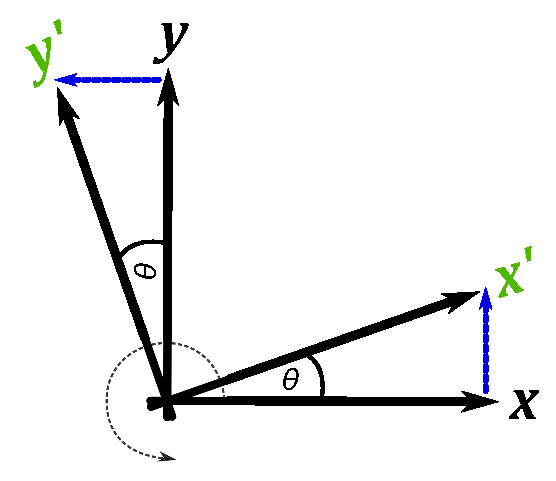
\includegraphics[scale=0.8]{inf-rot.eps}
\end{center}
  \caption{\label{fig:inf-rot}
A rotation of the coordinate axes around the $\hat z$ axis.}
\end{figure}
%

Note that this only works for infinitesimal rotation since for a finite rotation there will be contributions from multiple axes, \eg $\vec \delta x \propto \hat y - \hat x$, if you can't see this just remember the rotation matrix in 2 dimension.

How about a generic rotation axis? say we pick an arbitrary rotation axis $\vec r$ and we want to rotate a vector $\vec A$, remember that the magnitude of $\vec r$ is the amount of rotation, \ie
\nbea
\vec r = a \hat x + b \hat y + c \hat z &\longrightarrow& |\vec r| = \sqrt{a^2 + b^2 + c^2} = \epsilon
\neea

Thus the change in $\vec A$ is given by
\nbea
\vec \delta \vec A = \vec r \times \vec A & = & a (\hat x \times \vec A) + b (\hat y \times \vec A) + c (\hat z \times \vec A)
\neea

Here we see why it only works for infinitesimal rotations since rotations w.r.t different axes do not commute but they only contribute at $\epsilon^2$.

What if instead of a vector we have a scalar $A$? First we need to convert it into a vector, but how? there are many ways of doing it. If we look back to translation $A(x) \rightarrow A(x + \epsilon)$ the transformation we get is $A \rightarrow A + \epsilon \partial A$. Now, we just need to turn this into a vector, the most obvious way is $A \rightarrow A + \vec\epsilon \cdot  (\vec \nabla A)$ (note: we always need a derivative to calculate $\delta A$ thanks to taylor expansion).

Using the formula we have above 
\nbea
\vec \delta (\nabla A) = \vec r \times \nabla A & = & a (\hat x \times \nabla A) + b (\hat y \times \nabla A) + c (\hat z \times \nabla A)
\neea
however the result we have is a vector we need a scalar since $A$ was initially a scalar. The solution is just to take a dot product with $\vec x = \frac{1}{\sqrt{3}}(\hat x + \hat y + \hat z)$
\nbea
\delta A = \vec x \cdot (\vec r \times \nabla A) & = & - \vec r \cdot (\vec x \times \nabla A)
\neea
by using a triple scalar product rule, the thing here now is that I don't know how to get rid of that minus sign LOL

So for a general scalar field you'll get $\delta \phi = \vec \epsilon \cdot (\vec x \times \nabla) \phi$, sans a minus sign, where $\vec x$ is just the coordinate axes and $\vec \epsilon$ is the magnitude and axis of rotation.

Now, how does the lagrangian change? Well, the lagrangian is also a scalar quantity thus we can expect it to also change as $\delta \mathcal{L} =  \vec \epsilon \cdot (\vec x \times \nabla) \mathcal{L}$.

The goal here is to show that $\delta \mathcal{L}$ is related to the stress energy tensor {\it of translation} and for simplicity we will ignore $\vec \epsilon \cdot$ for now
\nbea
(\vec x \times \nabla) \mathcal{L} & = & \epsilon^{ijk} x_j \partial_k \mathcal{L} = \partial_\mu (\epsilon^{ijk} x_j \delta^\mu_k \mathcal{L}) \\
& = & \partial_\mu \mathcal{F}^{\mu i} \\
\rightarrow \mathcal{F}^{\mu i} & = & \epsilon^{ijk} x_j \delta^\mu_k \mathcal{L}
\neea
Since this is a symmetry the change must be a total derivative.

Now from the generic formula for energy stress tensor (under rotation)
\nbea
\widetilde T^{\mu i} & = & \frac{\delta \mathcal{L}}{\delta(\partial_\mu \phi)} \delta \phi - \mathcal{F}^{\mu i} \\
& = & \frac{\delta \mathcal{L}}{\delta(\partial_\mu \phi)} (\vec x \times \vec \nabla) \phi - \epsilon^{ijk} x_j \delta^\mu_k \mathcal{L} \\
& = & \epsilon^{ijk} x_j \left (  \frac{\delta \mathcal{L}}{\delta(\partial_\mu \phi)} \partial_k \phi - \delta^\mu_k \mathcal{L} \right ) =  \epsilon^{ijk} x_j (T^\mu_k) \\
& = & \vec x \times \vec T^\mu
\neea

Notes on energy stress tensor:
Under symmetry transformations, the lagrangian should change by a total derivative (since a symmetry should not change the physics)
\nbea
\delta\mathcal{L} & = & \partial_\mu \mathcal{F}^\mu
\neea 

However the transformation is also given by
\nbea
\delta\mathcal{L} & = & \frac{\delta \mathcal{L}}{\delta\phi}\delta \phi + \frac{\delta \mathcal{L}}{\delta(\partial_\mu \phi)} \delta(\partial_\mu \phi) \\
& = & \partial_\mu \left ( \frac{\delta \mathcal{L}}{\delta(\partial_\mu \phi)} \right ) \delta \phi + \frac{\delta \mathcal{L}}{\delta(\partial_\mu \phi)} \partial_\mu(\delta\phi) \\
\partial_\mu \mathcal{F}^\mu & = & \partial_\mu \left ( \frac{\delta \mathcal{L}}{\delta(\partial_\mu \phi)} \delta \phi \right ) \\
0 & = & \partial_\mu \left ( \frac{\delta \mathcal{L}}{\delta(\partial_\mu \phi)} \delta \phi - \mathcal{F}^\mu \right ) = \partial_\mu J^\mu \\
\rightarrow J^\mu & = & \frac{\delta \mathcal{L}}{\delta(\partial_\mu \phi)} \delta \phi - \mathcal{F}^\mu
\neea
where we have used the equation of motion on the first term going into the second line, this is actually tricky if we apply wrongly we will get something like (doing Integration by parts on the second term at the same time)
\nbea
\delta\mathcal{L} & = & \frac{\delta \mathcal{L}}{\delta\phi}\delta \phi + \frac{\delta \mathcal{L}}{\delta(\partial_\mu \phi)} \delta(\partial_\mu \phi) = \frac{\delta \mathcal{L}}{\delta\phi}\delta \phi - \partial_\mu \left ( \frac{\delta \mathcal{L}}{\delta(\partial_\mu \phi)} \right ) \delta \phi \\
& = & \partial_\mu \left ( \frac{\delta \mathcal{L}}{\delta(\partial_\mu \phi)} \right ) \delta \phi  - \partial_\mu \left ( \frac{\delta \mathcal{L}}{\delta(\partial_\mu \phi)} \right ) \delta \phi \\
& = & 0 ~~~ ???
\neea
LOL indeed but what went wrong? One, we can't really use IBP here since we are not really under an integral. However we can just use the usual trick, $u(dv) = d(uv) - (du)v$
\nbea
\frac{\delta \mathcal{L}}{\delta\phi}\delta \phi + \frac{\delta \mathcal{L}}{\delta(\partial_\mu \phi)} \delta(\partial_\mu \phi) & = & \frac{\delta \mathcal{L}}{\delta\phi}\delta \phi + \partial_\mu \left ( \frac{\delta \mathcal{L}}{\delta(\partial_\mu \phi)} \delta \phi \right ) - \partial_\mu \left ( \frac{\delta \mathcal{L}}{\delta(\partial_\mu \phi)} \right ) \delta \phi \\
& = & \left \{ \frac{\delta \mathcal{L}}{\delta\phi}\delta \phi - \partial_\mu \left ( \frac{\delta \mathcal{L}}{\delta(\partial_\mu \phi)} \right ) \delta \phi \right \} + \partial_\mu \left ( \frac{\delta \mathcal{L}}{\delta(\partial_\mu \phi)} \delta \phi \right ) \\
& = & 0 + \partial_\mu \left ( \frac{\delta \mathcal{L}}{\delta(\partial_\mu \phi)} \delta \phi \right )
\neea
again using the equations of motion for $\phi$.


-=-=-=-=-=-=-=-=-=-=-=-=-=-=-=-=-=-=-=-=-=-=-=-=-=-=-=-=-

In QFT, why does $\phi(x)$ create a particle at spacetime point $x$, \ie $\phi(x)| 0 \rangle = |x \rangle$? For simplicity we'll set $t = 0 \rightarrow \phi(x) = \phi(\vec x, 0)$. To see this take the inner product of
\nbea
\langle \vec x | \vec p \rangle & = & \langle 0 |\phi^\dagger(\vec x, 0) | \vec p \rangle \\
& = & \langle 0 | \left ( \int \frac{d^3 p'}{(2 \pi)^3 \sqrt{\omega_{p'}}} a^\dagger e^{-i\vec {p'} \vec x} +  a e^{i\vec {p'} \vec x} \right ) | \vec p \rangle \\
& = & \left ( \langle 0 | \int \frac{d^3 p'}{(2 \pi)^3 \sqrt{\omega_{p'}}} a e^{i\vec {p'} \vec x} \right ) | \vec p \rangle, ~~~ ( \langle 0 | a^\dagger ) = 0 \\
& = & \int \frac{d^3 p'}{(2 \pi)^3 \sqrt{\omega_{p'}}} e^{i\vec {p'} \vec x} ~~ \{ \langle \vec {p'} | \vec p \rangle \} \\
& = & \int \frac{d^3 p'}{(2 \pi)^3 \sqrt{\omega_{p'}}} e^{i\vec {p'} \vec x} ~~ \left \{ (2 \pi)^3 \sqrt{\omega_{p}} \delta (\vec {p'} - \vec p) \right \} \\
\langle \vec x | \vec p \rangle & = & e^{i\vec {p} \vec x}
\neea
Thus $\phi(x)$ does indeed create a particle at spacetime point $x$ :)

-=-=-=-=-=-=-=-=-=-=-=-=-=-=-=-=-=-=-=-=-=-=-=-=-=-=-=-=-

What is the explicit formula for multiple integrations of a function, \ie what is $\int\int ... \int f(x) dx$ ? The answer is the Cauchy formula for repeated integration
\nbea
(J f)(x) & = & \int_0^x f(t) dt \\
(J^2 f)(x) & = & \int_0^x \left ( \int_0^t f(s) ds \right ) dt \\
(J^\alpha f)(x) & = & \frac{1}{(\alpha - 1)!}\int_0^x (x - t)^{\alpha-1} f(t) dt \\
& = & \frac{1}{\Gamma(\alpha)}\int_0^x (x - t)^{\alpha-1} f(t) dt
\neea
Here we have used $J$ as an integration operator and the identity $\Gamma(\alpha) = (\alpha-1)!$, and also that gamma function can take non integer arguments compared to factorials.

So how do we derive this? The most intuitive derivation I saw was using Laplace transform, some preliminary Laplace transforms that we need are

1. Laplace transform of an integral of a function, $\mathcal{L}\{\int_0^x f(t) dt\}$
\nbea
\mathcal{L}\left \{\int_0^x f(t) dt \right \} & = & \int_0^\infty e^{-sx} \left ( \int_0^x f(t) dt \right ) dx
\neea
we now use integration by parts, $u = \left ( \int_0^x f(t) dt \right ),~dv = e^{-sx} dx $ such that
\nbea
\mathcal{L}\left \{\int_0^x f(t) dt \right \} & = &  \left. \left ( \int_0^x f(t) dt \right ) \frac{e^{-sx}}{(-s)} \right |_{x = 0}^{x = \infty} - \left ( -\frac{1}{s} \right ) \int_0^\infty e^{-sx} f(x) dx \\
& = & 0 + \frac{1}{s} \int_0^\infty e^{-sx} f(x) dx \\
\mathcal{L}\left \{ (J f) (x) \right \} & = & \frac{1}{s}\mathcal{L}\left \{ f(x) \right \} 
\neea
the boundary terms are zero because $\int_0^0 f(t) = 0$ and $e^{-\infty}=0$, assuming $f(t)$ is well behaved. Generalizing to $(J^\alpha f)(x)$ we have
\nbea
\mathcal{L}\left \{ (J^\alpha f) (x) \right \} & = & \frac{1}{s^\alpha}\mathcal{L}\left \{ f(x) \right \} 
\neea

2. Laplace transform of $x^\alpha$, \ie $\mathcal{L}\{x^\alpha\}$ (all function under Laplace transform are assumed to be valid only on the positive real axis)
\nbea
\mathcal{L}\left \{x^\alpha\right \} & = & \int_0^\infty e^{-sx} x^\alpha dx
\neea
here we just need to do multiple integration by parts with $u = x^\alpha,~dv = e^{-sx} dx$
\nbea
\mathcal{L}\left \{x^\alpha\right \} & = &  \left. x^\alpha e^{-sx} \right |_{x=0}^{x=\infty} - \frac{\alpha}{(-s)}\int_0^\infty x^{\alpha-1} e^{-sx} dx \\
& = & \frac{\alpha}{s}\int_0^\infty x^{\alpha-1} e^{-sx} dx
\neea
here we can do 2 things, one use the definition of gamma function $\Gamma(\alpha) = \int_0^\infty x^{\alpha-1} e^{-x} dx$ or repeat the integration by parts again (note that the boundary terms are again zero in this case), if we repeat the IBP $\alpha-1$ more times we get
\nbea
\mathcal{L}\left \{x^\alpha\right \} & = & \frac{\alpha !}{s^\alpha}\int_0^\infty e^{-sx} dx \\
& = & \left. \frac{\alpha !}{s^\alpha} \frac{1}{(-s)} e^{-sx} \right |_{0}^{\infty} \\
& = & -\frac{\alpha !}{s^{\alpha+1}} \left ( e^{-\infty}- e^0\right ) \\
\mathcal{L}\left \{x^\alpha\right \}  & = & \frac{\alpha !}{s^{\alpha+1}}
\neea
which can be generalized to $\mathcal{L}\left \{x^\alpha\right \}  = \frac{\Gamma(\alpha+1)}{s^{\alpha+1}}$ {\it or} just by using the definition of gamma function from the beginning
\nbea
\frac{\alpha}{s}\int_0^\infty x^{\alpha-1} e^{-sx} dx & = & \frac{\alpha}{s}\int_0^\infty \left (\frac{y}{s}\right )^{\alpha-1} e^{-y} \left (\frac{dy}{s} \right), ~~~ y = sx,~ dx = \frac {dy}{s}\\
& = & \frac{\alpha}{s^{\alpha+1}}\int_0^\infty y^{\alpha-1} e^{-y} dy = \frac{\alpha \Gamma(\alpha)}{s^{\alpha+1}},~~~ \alpha \Gamma(\alpha) = \Gamma(\alpha+1)\\
\mathcal{L}\left \{x^\alpha\right \} & = & \frac{\Gamma(\alpha + 1)}{s^{\alpha+1}}
\neea
which is the same result as above.

3. The infamous convolution formula 
\nbea
\mathcal{L}\{f\}\mathcal{L}\{g\} & = & \left (\int_0^\infty e^{-sx} f(x) dx\right )\left (\int_0^\infty e^{-sy} g(y) dy\right ) \\
& = & \int_0^\infty e^{-s(x+y)}  \left ( \int_0^{\infty} f(x) g(y) dy \right ) dx, ~~~ z = x + y \\
& = & \int_0^\infty e^{-s z} \left ( \int_0^{z} f(z-y) g(y) dy \right ) dz \\
\mathcal{L}\{f\}\mathcal{L}\{g\} & = & \mathcal{L} \{ f * g\}
\neea
where $*$ denotes convolution, some explanation on $dx \rightarrow dz$, inside the brackets of $\int dy$, $x$ is constant while outside of this bracket $y$ is {\it constant} and thus $dz = dx$.
 
We are now ready to derive the formula for $(J^\alpha f)(x)$
\nbea
(J^\alpha f)(x) & = & \mathcal{L}^{-1} \{ \mathcal{L} \{J^\alpha f\} \} \\
& = & \mathcal{L}^{-1} \left \{ \frac{1}{s^\alpha} \mathcal{L} \{ f\} \right \} = \mathcal{L}^{-1} \left \{ \frac{\Gamma(\alpha)}{\Gamma(\alpha)}\frac{1}{s^\alpha} \mathcal{L} \{ f\} \right \} \\
& = & \frac{1}{\Gamma(\alpha)}\mathcal{L}^{-1} \left \{ \frac{\Gamma(\alpha)}{s^\alpha} \mathcal{L} \{ f\} \right \} \\
& = & \frac{1}{\Gamma(\alpha)} \left ( \mathcal{L}^{-1} \left \{ \frac{\Gamma(\alpha)}{s^\alpha} \right \} *  f \right ) \\
& = & \frac{1}{\Gamma(\alpha)} \left ( x^{\alpha-1} *  f \right ) \\
(J^\alpha f)(x) & = & \frac{1}{\Gamma(\alpha)} \int_0^x ( x - t )^{\alpha-1}  f(t) dt 
\neea
which is the Cauchy formula we were looking for.

===========================================================

Problem 1.1 Srednicki, Show that the Dirac matrices must be even dimensional. Hint: show that the eigenvalues of $\beta$ are all $\pm 1$, and that ${\rm Tr} \beta = 0$. To show that ${\rm Tr} \beta = 0$, consider \eg ${\rm Tr} \alpha_1^2 \beta$. Similarly, show that ${\rm Tr} \alpha_i = 0$.

Some facts about Dirac matrices
%
\nbea
\{ \alpha^j, \alpha^k\}_{ab} = 2\delta^{jk}\delta_{ab} ~~~ \{ \alpha^j, \beta\}_{ab} = 0 ~~~ (\beta)^2_{ab} = \delta_{ab}
\neea
%
For eigenvalues of $\beta$ it follows immediately from $(\beta)^2_{ab} = \delta_{ab}$ its eigenvalues must be $\pm 1$.

For ${\rm Tr} \beta$ we start with
%
\nbea
{\rm Tr} (\alpha_1^2 \beta) & = & {\rm Tr} (\alpha_1 \beta \alpha_1), ~~\{ \alpha^j, \beta\}_{ab} = 0 \\
& = & {\rm Tr} (-\beta \alpha_1 \alpha_1) \\
{\rm Tr} (\alpha_1^2 \beta) & = & {\rm Tr} (\beta  \alpha_1 \alpha_1), ~~{\rm Tr}(AB) = {\rm Tr}(BA) \\
\rightarrow {\rm Tr} (-\beta \alpha_1 \alpha_1) & = & {\rm Tr} (\beta \alpha_1 \alpha_1) \\
{\rm Tr} (\beta \alpha_1 \alpha_1) & = & 0
\neea
%
Now from $\{ \alpha^j, \alpha^k\}_{ab} = 2\delta^{jk}\delta_{ab} \rightarrow \{ \alpha_i, \alpha_i\}_{ab} = 2 \delta_{ab}$, it means that $(\alpha^2_i)_{ab} = \delta_{ab}$ and thus ${\rm Tr} (\beta \alpha_i \alpha_i) = {\rm Tr} (\beta) = 0$.

Now since ${\rm Tr} \beta = 0$ and its eigenvalues are $\pm 1$, $\beta$ must be even dimensional.

This argument applies for ${\rm Tr} \alpha_i$ as well by reversing the roles of $\beta$ and $\alpha$, ${\rm Tr} (\beta^2 \alpha_i) = {\rm Tr} (\alpha_i) = 0$ and since $(\alpha^2_i)_{ab} = \delta_{ab} \rightarrow$ eigenvalues must be $\pm 1$, $\alpha^i$ must be even dimensional. This means that {\it all} of Dirac matrices must be even dimensional.

Now we need to show that Dirac matrices must be bigger than $2 \times 2$. I'll start with the fact that any $2 \times 2$ matrix can be written as $ a_0 1 + a_i \sigma^i$, \ie a combination of Pauli matrices and the identity matrix. If you remember some sort of group theory, the group $su(2)$ spans a three sphere and the basis vectors (lie algebra $SU(2)$) are spanned by the Pauli matrices.

The commutation relations of Pauli matrices are
%
\nbea
\{\sigma^i, \sigma^j\}_{ab} & = & 2\delta^{ij} \delta_{ab} \\
\lbrack \sigma^i, \sigma^j \rbrack & = & 2 i \varepsilon^{ijk} \sigma^{k} 
\neea
%
As we can see from their anticommutation relations, the pauli matrices can play the role of $\alpha^i$. We now need to show that there are no fourth $2\times2$ matrix to play the role of $\beta$. To do this let's construct a generic $2\times2$ matrix $A = a_0 1 + a_i \sigma^i$ and do its commutation relation with the pauli matrices and see what coefficients $(a_0, a_i)$ we need to fulfill the commutation relation $\{ \alpha^j, \beta\}_{ab} = 0$
%
\nbea
\{A, \sigma^j\} & = & \{a_0 1 + a_i \sigma^i,  \sigma^j\} \\
0 & = & \{a_0 1,  \sigma^j\}  + \{a_i \sigma^i,  \sigma^j\} \\
0 & = & 2 a_0 \sigma^j + a_i \delta^{ij} 1 \\
0 & = & 2 a_0 \sigma^j + a_j 1
\neea
%
Recall that there's only one diagonal pauli matrix, \ie if you use $\hat z$ as the main direction $\sigma_z = (+1, -1)$ which is just spin up and spin down and the other two pauli matrices will be off diagonal, if you choose any other axis the same will occur, only one will be diagonal and the other two will be off diagonal.

From $0 = 2 a_0 \sigma^j + a_j 1$, we need $\sigma^j$ to be diagonal but since $\sigma^j = (+1, -1)$ the only solution is $a_0 = 0, a_j = 0$. However the anticommutation relation $\{A, \sigma^j\} = 0$ has to be true for all values of $j = 1,2,3$ which means that $a_1 = a_2 = a_3 = 0 \rightarrow A = 0$, so the only $2\times2$ matrix that can fulfill the role of $\beta$ is the zero matrix. However, $\beta^2 = 1$, hence Dirac matrices must be at least $4\times4$.

===============================================================

Srednicki Problem 4.1 Verify eq. (4.12). Verify its limit as $m \rightarrow 0$. Eq. 4.12 is $\lbrack \varphi^+(x),\varphi^-(x') \rbrack = (m/4\pi^2 r) K_1(mr) \equiv C(r)$ where $K_1(mr)$ is a modified Bessel function of the second kind.

The subject here is that for a transition amplitude to be Lorentz invariance, the above commutator must be zero, however it's not. Why does it have to be zero? because the transition amplitude is given by time ordered product of the fields and for spacelike separations, $x-x' > 0$, the time ordering might shuffle the order of the fields as for a spacelike separation different observers might see two events happen in different orders. Note that the metric used here is $(-+++)$. Hence the need to set $\lbrack \varphi^+(x),\varphi^-(x') \rbrack = 0$ to maintain equal transition amplitudes for all observers, $\langle \varphi(x) \varphi(y) \rangle = \langle \varphi(y) \varphi(x) \rangle$.

However, eq. 4.12 shows that $\lbrack \varphi^+(x),\varphi^-(x') \rbrack \neq 0$! Our task at hand is to derive this conclusion. First we need to choose a frame where $t-t'=0$ as suggested by the text to simplify calculation.
%
\nbea
\int \widetilde{dk} ~e^{ik(x-x')} & = & \int \frac{d^3k}{(2 \pi)^3 2 \sqrt{k^2 + m^2}} e^{(-ik_0 \Delta t + i \vec k \cdot \Delta \vec x)}, ~\Delta t = 0 \\
& = &  \int \frac{d^3k}{(2 \pi)^3 2 \sqrt{k^2 + m^2}} e^{(i\vec k \cdot \Delta \vec x)}\\
& = &  \int \frac{d^3k}{(2 \pi)^3 2 \sqrt{k^2 + m^2}} e^{i|k||r| \cos \theta}, ~ |r| = |\Delta \vec x|\\
& = &  \int \frac{k^2 dk~ d\phi~ d(\cos\theta)} {(2 \pi)^3 2 \sqrt{k^2 + m^2}} e^{i|k||r| \cos \theta}\\
& = &  \int \frac{k^2 dk~ \bcancel{2 \pi}} {(2 \pi)^{\bcancel{3}2} 2 \sqrt{k^2 + m^2}} \int^1_{-1} d(\cos\theta)~e^{i|k||r| \cos \theta}\\
& = &  \int \frac{k^2 dk} {(2 \pi)^2 2 \sqrt{k^2 + m^2}} \frac{(e^{i|k||r|} - e^{-i|k||r|})}{ikr}\\
& = &  \int \frac{k dk} {(2 \pi)^2 \bcancel{2} \sqrt{k^2 + m^2}} \frac{\bcancel{2}\bcancel{i}\sin(k r)}{\bcancel{i}r}\\
& = &  \frac{1} {(2 \pi)^2 r} \int_0^\infty dk \frac{k \sin(k r)} {\sqrt{k^2 + m^2}} 
\neea
%
We now need to massage this into a Bessel function, but first let's do a change of variable $ \rightarrow y = k/m$
%
\nbea
& = &  \frac{1} {(2 \pi)^2 r}  \int_0^\infty m ~d\left(\frac{k}{m}\right) \frac{m \left(\frac{k}{m}\right) \sin(\left(\frac{k}{m}\right) m r)} {m \sqrt{\left(\frac{k}{m}\right)^2 + 1}} \\
& = &  \frac{m} {(2 \pi)^2 r}  \int_0^\infty dy \frac{y \sin(y m r)} {\sqrt{y^2 + 1}} 
\neea
%
now, there are 2 facts we need about Bessel functions
%
\nbea
K_0(z) & = & \int_0^\infty dy \frac{\cos(zy)}{\sqrt{y^2 + 1}} \\
\frac{d}{dz} K_\nu(z) & = & \frac{\nu}{z} K_{\nu}(z) - K_{\nu+1}(z) \\
\rightarrow \frac{d}{dz} K_0(z) & = & - K_{1}(z)
\neea
%
If we do the actual derivative on $K_0$ we get
%
\nbea
\rightarrow \frac{d}{dz} K_0(z) & = & \int_0^\infty dy \frac{d}{dz} \left (\frac{\cos(zy)}{\sqrt{y^2 + 1}} \right ) \\
- K_{1}(z) & = & - \int_0^\infty dy \frac{y \sin(zy)}{\sqrt{y^2 + 1}} \\
\rightarrow \frac{m} {(2 \pi)^2 r} K_{1}(z) & = & \frac{m} {(2 \pi)^2 r} \int_0^\infty dy \frac{y \sin(zy)}{\sqrt{y^2 + 1}}, ~ z \rightarrow mr \\
\frac{m} {4 \pi^2 r} K_{1}(mr) & = & \frac{m} {(2 \pi)^2 r} \int_0^\infty dy \frac{y \sin(mr y)}{\sqrt{y^2 + 1}} \\
\frac{m} {4 \pi^2 r} K_{1}(mr) & = & \int \widetilde{dk} ~e^{ik(x-x')}
\neea
%
and that is the result that we want. How about its limit as $m \rightarrow 0$? One might be tempted to find or calculate the power series expansion of the Bessel function around $z \rightarrow 0$ but I found it extremely difficult (as I've forgotten most of the methods from my mathematical methods class) but (after looking at the problem long enough) I realized that we need not mess with Bessel functions at all.

You see $\int \widetilde{dk} ~e^{ik(x-x')}$ looks a lot like a fourier transform and setting $m \rightarrow 0$ makes it look like this
%
\nbea
& = &  \int \frac{d^3k} {(2 \pi)^3 2 \sqrt{k^2 + m^2}} e^{i \vec k \cdot \vec r}, ~m \rightarrow 0\\
& = &  \frac{1}{2 (2 \pi)^3} \int d^3k \frac{e^{i \vec k \cdot \vec r}}{|k|}
\neea
%
which looks a lot like the fourier transform of the Coulomb potential but this time it's going into the $\vec x$ domain instead of the $\vec k$ domain.

The evaluation of this integral is usually done using a regulator $e^{-\mu k}$ and we'll take the limit $\mu \rightarrow 0$ at the end.
%
\nbea
& = & \frac{1}{2 (2 \pi)^3} \int d^3k \frac{e^{-\mu k} e^{i \vec k \cdot \vec r}}{|k|} \\
& = & \frac{1}{2 (2 \pi)^3} \int k^{\bcancel{2}} dk ~ d\phi~ \frac{e^{-\mu k}}{\bcancel{k}} \int_{-1}^1 d(\cos\theta) e^{i |k| |r| \cos \theta} \\
& = & \frac{1}{2 (2 \pi)^2} \int_0^\infty \bcancel{k} dk ~ e^{-\mu k} \frac{(e^{i k r} - e^{-i k r})}{i \bcancel{k} r} \\
& = & \frac{1}{2 i r (2 \pi)^2} \int_0^\infty dk ~ e^{-\mu k} (e^{i k r} - e^{-i k r}) \\
& = & \frac{1}{2 i r (2 \pi)^2} \left \lbrack \frac{1}{(-\mu + ir)} \left. e^{(-\mu + i r)k} \right |_0^\infty - \frac{1}{(-\mu - ir)} \left. e^{(-\mu - i r)k} \right |_0^\infty \right \rbrack \\
& = & \frac{1}{2 i r (2 \pi)^2} \left \lbrack \frac{1}{(-\mu + ir)} (e^{-\infty} - e^0 ) - \frac{1}{(-\mu - ir)} (e^{-\infty} - e^0 ) \right \rbrack \\
& = & \frac{1}{2 i r (2 \pi)^2} \left \lbrack \frac{1}{(-\mu - ir)} - \frac{1}{(-\mu + ir)} \right \rbrack =  \frac{1}{2 i r (2 \pi)^2} \left \lbrack \frac{-\mu + ir + \mu + ir}{\{(-\mu)^2 - (ir)^2\}} \right \rbrack \\
& = & \frac{1}{\bcancel{2 i r} (2 \pi)^2} \frac{\bcancel{2 i r}}{\{(-\mu)^2 + r^2\}}, ~\mu \rightarrow 0 \\
& = & \frac{1}{4 \pi^2 r^2}
\neea
%
which is the result we want :) without messing with Bessel functions at all

===============================================================

How do you do the integral of $\int_{-\infty}^{\infty} dx \frac{\sin x}{x}$? The common solution is to do a contour integration, but is there another way? This was what I attempted, the answer to that question is in short no, but I sure learned a hell lot thinking about this problem.

First, there's no function whose derivative is $\frac{\sin x}{x}$ which means that the indefinite integral $\int dx \frac{\sin x}{x}$ has no solution. Contour integral was a neat technique apropos to a numerical calculation.

My original approach was inspired by green's function method. This was because the integral $\int dx \frac{\sin x}{x}$ is akeen to $\int dk \frac {e^{ikx}}{k}$ and since $\cos k$ is even, only the $\sin k$ term will survive the integration $\rightarrow \int dk \frac {i\sin (kx)}{k}$ and by taking $x \rightarrow 1$ we'll get $\int dk \frac{i \sin k}{k}$ which is what we want. The starting point is the unit step function $u(x)$
%
\nbea
\frac{d}{dx} u(x) & = & \delta(x) \\
\rightarrow ik ~ u(k) & = & 1 \\
u(k) & = & \frac{1}{ik}
\neea
%
We must take a pause here. First some trivial things, I have chosen the fourier transform pair to be $f(x) = \frac{1}{2\pi} \int dk e^{ikx} F(k)$ and $F(k) = \int dx e^{-ikx} f(x)$, \ie we put all factor of normalization $\frac{1}{2\pi}$ in the inverse transform. We can choose other normalization schemes, but the result will be the same.

The second reason to pause here is more serious. The unit step function is a peculiar function. Note that
%
\nbea
\frac{d}{dx}  \left ( u(x) + C \right ) & = & \delta(x)
\neea
%
is still true for any constant $C$. But there's a particular value of $C$ that has serious ramifications, \ie $C = -\frac{1}{2}$. Why? because
%
\nbea
\left (u(x) - \frac{1}{2} \right ) & = & \frac{1}{2} \left ( u(x) - u(-x) \right )
\neea
%
that is $\left (u(x) - \frac{1}{2} \right )$ is just the antisymmetric part of $u(x)$. Now there is a fact that we need to remember, an antisymmetric (real) function has as its fourier counterpart a purely imaginary function $\int dx e^{-ikx} f(x) = -i\int dx \sin(kx) f(x)$. We see above that $u(k) = \frac{1}{ik}$ (purely imaginary) and since $\frac{d}{dx} u(x) = \frac{d}{dx}  \left ( u(x) + C \right )$ what we were really doing was fourier transforming only the antisymmetric part of $u(x)$, \ie
%
\nbea
\frac{d}{dx}  \left ( \frac{1}{2} (u(x) - u(-x)) \right ) & = & \frac{d}{dx}  \left ( u(x) - \frac{1}{2} \right )  = \delta(x) \\
\mathcal{F}\left \{ \frac{d}{dx}  \left ( u(x) - \frac{1}{2} \right ) \right \} & = & \mathcal{F}\left \{ \delta(x) \right \} \\
ik ~\mathcal{F} \left \{ \left ( u(x) - \frac{1}{2} \right ) \right \} & = & 1 \\
ik \left ( u(k) - \frac{1}{2} (2\pi \delta(k)) \right ) & = & 1 \\
u(k) & = & \frac{1}{ik} + \pi \delta(k)
\neea
%
Note that $\mathcal{F}\left \{ \delta(x) \right \} = 1$ and $\mathcal{F}\left \{ 1 \right \} = 2\pi \delta(k)$ is affected by the normalization scheme, other schemes will produce different numerical factors. Now, what does it have to do with $\int dx \frac{\sin x}{x}$? Let's do an inverse fourier transform on the above function
%
\nbea
\mathcal{F}^{-1}\left \{ u(k) \right \} & = & \mathcal{F}^{-1}\left \{ \frac{1}{ik} + \pi \delta(k) \right \} \\
u(x) & = & \frac{1}{2\pi} \int_{-\infty}^{\infty} dk \frac{e^{ikx}}{ik} + \frac{1}{2\bcancel{\pi}} \int_{-\infty}^{\infty} dk~e^{ikx} \left ( \bcancel{\pi} \delta(k) \right ) \\
u(x) & = & \frac{1}{2\pi i} \int_{-\infty}^{\infty} dk \frac{e^{ikx}}{k} + \frac{1}{2}
\neea
%
Now we set $x \rightarrow 1, u(1) = 1$
%
\nbea
u(1) & = & \frac{1}{2\pi i} \int_{-\infty}^{\infty} dk \frac{e^{ik}}{k} + \frac{1}{2} \\
1 & = & \frac{1}{2\pi \bcancel{i}} \int_{-\infty}^{\infty} dk \frac{\bcancel{i} \sin k}{k} + \frac{1}{2} \\
\rightarrow \int_{-\infty}^{\infty} dk \frac{\sin k}{k} & = & \pi
\neea
%
In the second line we have used the fact that since $\frac{\cos k}{k}$ is an odd function, its integral is zero. And this is the origin of the factor of $\pi$. For the longest time I have wondered how this integral has anything to do with $\pi$. But wait, you might ask how in turn did the fourier transform pair acquire this factor of $\frac{1}{2\pi}$ in the first place?

The answer to that question is the gaussian integral $e^{-x^2/2}$. This gaussian function is the eigenfunction of the fourier transform. Let's see how it works
%
\nbea
\int_{-\infty}^{\infty} dx~ e^{-ikx} e^{-x^2/2} & = & \sqrt{2 \pi} ~e^{\frac{(-ik)^2}{4\left( \frac{1}{2} \right)}} \\
& = & \sqrt{2 \pi} ~e^{-k^2/2}
\neea
%
where we have used the gaussian integral formula $\int dx~e^{-ax^2 + bx + c} = \sqrt{\frac{\pi}{a}} e^{\frac{b^2}{4a} + c}$ and if we do an inverse transform we get
%
\nbea
\int_{-\infty}^{\infty} dk~ e^{ikx} \left ( \sqrt{2 \pi} ~e^{-k^2/2} \right ) & = & \sqrt{2 \pi}\sqrt{2 \pi}~ e^{\frac{(ix)^2}{4\left( \frac{1}{2} \right)}} \\
& = & 2 \pi ~e^{-x^2/2}
\neea
%
Thus
%
\nbea
\mathcal{F}^{-1} \left \{ \mathcal{F} \left \{ e^{-x^2/2}\right \} \right \} & = & 2 \pi ~e^{-x^2/2}
\neea
%
or equivalently
%
\nbea
e^{-(0)^2/2} & \stackrel{\text{\tiny ?}}{=} & \int_{-\infty}^{\infty} dk~ e^{ik(0)} \left ( \sqrt{2 \pi} ~e^{-k^2/2} \right ) \\
& = & \sqrt{2 \pi} \int_{-\infty}^{\infty} dk~e^{-k^2/2} =  \sqrt{2 \pi} \sqrt{2 \pi} \\
1 & \stackrel{\text{\tiny ?}}{=} & 2 \pi
\neea
%
this means that we need to absorb the extra factor of $2 \pi$ somehow, the usual way is to put a $\frac{1}{2\pi}$ in the inverse transform, another common way is to put a factor of $\frac{1}{\sqrt{2 \pi}}$ on both the fourier transform and its inverse. Note that my derivation of $\int \frac{\sin k}{k}$ does not depend on the normalization scheme, you might try it if you don't believe me ;)

But then again, how did the gaussian integral get a factor of $\pi$, well it's because we use a circle to compute it, remember?
%
\nbea
\int_{-\infty}^{\infty} e^{-x^2/2} & = & \sqrt {\left ( \int_{-\infty}^{\infty} e^{-x^2/2} \int_{-\infty}^{\infty} e^{-y^2/2}\right ) } \\
& = & \sqrt { \int_{-\infty}^{\infty} dx dy ~ e^{-(x^2 + y^2)/2}} \\
& = & \sqrt { \left ( \int_0^{2\pi} d\phi \right )\int_{0}^{\infty} r dr  ~ e^{-(r^2)/2}} \\
\int_{-\infty}^{\infty} e^{-x^2/2} & = & \sqrt {2 \pi}
\neea
%
And that my friend, is how you get a factor of $\pi$ in the first place :) Of course in the contour integration of $\int \frac{\sin x}{x}$ the factor of $\pi$ is due to the infinitesimal semi circle around $x=0$ but again, it's all due to a circle.

It took me two days to figure this out and I learned a lot about the step function and fourier transform in the process. It all started with a simple thought of whether or not it's possible to compute $\int \frac{\sin x}{x}$ wihout contour integration, turns out that it's not quite possible, sometimes we do need a new technique to solve an old problem and I gained a new respect for complex numbers.

%how to strike out texts
%$\msout{\mathsf{stuckout}}$

%$\cancel{5}$

%$\bcancel{5}$

\end{document}
